% 本模板根据中国科学院大学本科生公共必修课程《基础物理实验》Word模板格式编写
% 本模板由Shing-Ho Lin和Jun-Xiong Ji于2022年9月共同完成, 旨在方便LaTeX原教旨主义者和被Word迫害者写实验报告, 避免Word文档因插入过多图与公式造成卡顿. 
% 如有任何问题, 请联系: linchenghao21@mails.ucas.ac.cn
% This is the LaTeX template for experiment report of Experimental Physics courses, based on its provided Word template. 
% This template is completed by the joint collabration of Shing-Ho Lin and Junxiong Ji in September 2022. 
% Adding numerous pictures and equations leads to unsatisfying experience in Word. Therefore LaTeX is better. 
% Feel free to contact us via: linchenghao21@mails.ucas.ac.cn

\documentclass[11pt]{article}

\usepackage[a4paper]{geometry}
\geometry{left=2.0cm,right=2.0cm,top=2.2cm,bottom=2.2cm}

\usepackage{ctex} % 支持中文的LaTeX宏包
\usepackage{amsmath,amsfonts,graphicx,subfigure,amssymb,bm,amsthm,mathrsfs,mathtools,breqn} % 数学公式和符号的宏包集合
\usepackage{algorithm,algorithmicx} % 算法和伪代码的宏包
\usepackage[noend]{algpseudocode} % 算法和伪代码的宏包
\usepackage{fancyhdr} % 自定义页眉页脚的宏包
\usepackage[framemethod=TikZ]{mdframed} % 创建带边框的框架的宏包
\usepackage{fontspec} % 字体设置的宏包
\usepackage{adjustbox} % 调整盒子大小的宏包
\usepackage{fontsize} % 设置字体大小的宏包
\usepackage{tikz,xcolor} % 绘制图形和使用颜色的宏包
\usepackage{multicol} % 多栏排版的宏包
\usepackage{multirow} % 表格中合并单元格的宏包
\usepackage{pdfpages} % 插入PDF文件的宏包
\RequirePackage{listings} % 在文档中插入源代码的宏包
\RequirePackage{xcolor} % 定义和使用颜色的宏包
\usepackage{wrapfig} % 文字绕排图片的宏包
\usepackage{bigstrut,multirow,rotating} % 支持在表格中使用特殊命令的宏包
\usepackage{booktabs} % 创建美观的表格的宏包
\usepackage{circuitikz} % 绘制电路图的宏包
\usepackage[inline]{enumitem}
\usepackage{tabularx}

\usepackage{indentfirst}
\setlength{\parindent}{2em}
\setlength{\abovecaptionskip}{2pt}
\setlength{\belowcaptionskip}{2pt}
\setlength{\intextsep}{8pt}
\setlength{\floatsep}{8pt}

\definecolor{dkgreen}{rgb}{0,0.6,0}
\definecolor{gray}{rgb}{0.5,0.5,0.5}
\definecolor{mauve}{rgb}{0.58,0,0.82}
\lstset{
  frame=tb,
  aboveskip=3mm,
  belowskip=3mm,
  showstringspaces=false,
  columns=flexible,
  framerule=1pt,
  rulecolor=\color{gray!35},
  backgroundcolor=\color{gray!5},
  basicstyle={\small\ttfamily},
  numbers=none,
  numberstyle=\tiny\color{gray},
  keywordstyle=\color{blue},
  commentstyle=\color{dkgreen},
  stringstyle=\color{mauve},
  breaklines=true,
  breakatwhitespace=true,
  tabsize=3,
}

% 轻松引用, 可以用\cref{}指令直接引用, 自动加前缀. 
% 例: 图片label为fig:1
% \cref{fig:1} => Figure.1
% \ref{fig:1}  => 1
\usepackage[capitalize]{cleveref}
% \crefname{section}{Sec.}{Secs.}
\Crefname{section}{Section}{Sections}
\Crefname{table}{Table}{Tables}
\crefname{table}{Table.}{Tabs.}

\setmainfont{Palatino Linotype.ttf}
\setCJKmainfont{SimHei.ttf}
% \setCJKsansfont{Songti.ttf}
% \setCJKmonofont{SimSun.ttf}
\punctstyle{kaiming}
% 偏好的几个字体, 可以根据需要自行加入字体ttf文件并调用

\renewcommand{\emph}[1]{\begin{kaishu}#1\end{kaishu}}

%改这里可以修改实验报告表头的信息
\newcommand{\experiName}{磁场的测量}
\newcommand{\supervisor}{丰家峰}
\newcommand{\name}{张欣培}
\newcommand{\studentNum}{2022K8009922001}
\newcommand{\class}{01}
\newcommand{\group}{10}
\newcommand{\seat}{3}
\newcommand{\dateYear}{2023}
\newcommand{\dateMonth}{12}
\newcommand{\dateDay}{11}
\newcommand{\room}{教708}
\newcommand{\others}{$\square$}
%% 如果是调课、补课, 改为: $\square$\hspace{-1em}$\surd$
%% 否则, 请用: $\square$
%%%%%%%%%%%%%%%%%%%%%%%%%%%

\begin{document}

%若需在页眉部分加入内容, 可以在这里输入
% \pagestyle{fancy}
% \lhead{\kaishu 测试}
% \chead{}
% \rhead{}

\begin{center}
    \LARGE \bf 《\, 基\, 础\, 物\, 理\, 实\, 验\, 》\, 实\, 验\, 报\, 告
\end{center}

\begin{center}
    \noindent \emph{实验名称}\underline{\makebox[25em][c]{\experiName}}
    \emph{指导教师}\underline{\makebox[8em][c]{\supervisor}}\\
    \emph{姓名}\underline{\makebox[6em][c]{\name}} 
    % 如果名字比较长, 可以修改box的长度"6em"
    \emph{学号}\underline{\makebox[10em][c]{\studentNum}}
    \emph{分班分组及座号} \underline{\makebox[5em][c]{\class \ -\ \group \ -\ \seat }\emph{号}} (\emph{例}:\, 1\,-\,04\,-\,5\emph{号})\\
    \emph{实验日期} \underline{\makebox[3em][c]{\dateYear}}\emph{年}
    \underline{\makebox[2em][c]{\dateMonth}}\emph{月}
    \underline{\makebox[2em][c]{\dateDay}}\emph{日}
    \emph{实验地点}\underline{{\makebox[4em][c]\room}}
    \emph{调课/补课} \underline{\makebox[3em][c]{\others\ 是}}
    \emph{成绩评定} \underline{\hspace{5em}}
    {\noindent}
    \rule[8pt]{17cm}{0.2em}
\end{center}

\begin{center}
    \Large \bf 第一部分\qquad 利用霍尔效应实验仪测量磁感应强度
\end{center}

\section{实验目的}

\begin{enumerate}
    \item 复习霍尔效应原理,了解霍尔元件有关参数的含义和作用
    \item 测绘霍尔元件的$V_H-I_S$,$V_H-I_M$ 曲线,了解霍尔电势差$V_H $与霍尔元件工作电流$I_S$、磁感应强度$B$ 及励磁电流$I_M$之间的关系。
    \item 学习利用霍尔效应测量磁感应强度$B$及磁场分布。
    \item 了解影响实验系统误差的霍尔元件因素和温差电动势因素,理解“对称交换测量法”的原理,学习用“对称交换测量法”消除负效应产生的系统误差。
\end{enumerate}

\section{实验器材}

    \hspace*{2em} 杭州大华DH4512D霍尔效应实验仪,万用表,台式万用表,信号发生器,导线等。
    \begin{figure}[H]
        \centering
        \begin{minipage}[t]{0.65\linewidth}
            \centering
            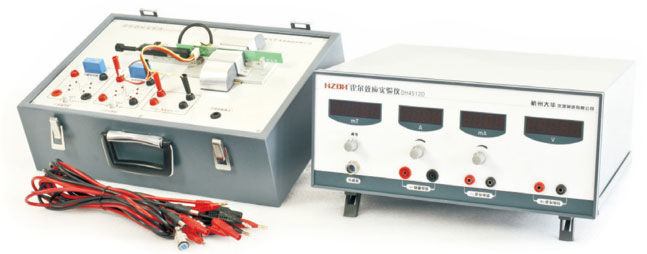
\includegraphics[width=10cm]{Fig/1.jpg}
            \caption{DH4512D霍尔效应实验仪}
        \end{minipage}
        \begin{minipage}[t]{0.34\linewidth}
            \centering
            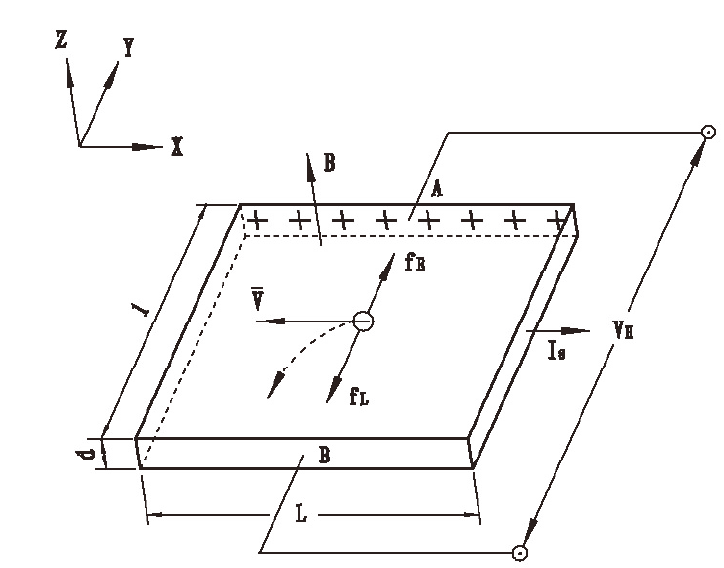
\includegraphics[width=5.5cm]{Fig/2.png}
            \caption{霍尔效应示意图}
            \label{fig:2}
        \end{minipage}
        
    \end{figure}
\section{实验原理}
\begin{enumerate}
    \item 霍尔效应
    \par \hspace*{2em}霍尔效应从本质上讲,是运动的带电粒子在磁场中受洛仑兹力的作用而引起的偏转。当带电粒子(电子或空穴)被约束在固体材料中,这种偏转就导致在垂直电流和磁场的方向上产生正负电荷在不同侧的聚积,从而形成附加的横向电场。
    \par \hspace*{2em}如图\cref{fig:2},磁场对电荷产生洛伦兹力$\mathbf{f_L=q\cdot(\bar{v}\times B)}$,电场对电荷产生电场力$\mathbf{f_E=qE_H=q\frac{V_H}{l}}$。其中,q为电荷携带的电荷量,对每个电子为-e;$\bar{v}$为电子漂移的平均速度矢量;$B$为磁感应强度,$E_H$为霍尔电场强度,$V_H$为霍尔电势,$l$为霍尔元件宽度。注意这两个运算是向量运算,有方向,两力恰好方向相反。当达到动态平衡时,$\mathbf{f_L+f_E}=0$。
    代入工作电流$I_S=ne\bar{v}ld$,其中厚度为d,载流子浓度为n,得
    \begin{equation}
        V_H=\frac{1}{ne}\frac{I_SB}{d}=R_H\frac{I_SB}{d}
    \end{equation}
    $R_H=\frac{1}{ne}$称为霍尔系数。代入材料的电导率$\sigma=ne\mu$,其中$\mu$为载流子的迁移率。得$R_H=\frac{\mu}{\sigma}$。
    \par \hspace*{2em}当霍尔元件的材料和厚度确定时,设:
    \begin{equation}
        K_H=\frac{R_H}{d}=\frac{l}{ned}\left[mV/(mA\cdot T)\right]
    \end{equation}
    $K_H$称为元件的灵敏度,它表示霍尔元件在单位磁感应强度和单位控制电流下的霍尔电势大小。一般要求$K_H$愈大愈好。
    \par \hspace*{2em}应当注意,磁感应强度不一定与霍尔片绝对垂直,作用在元件上的有效磁场是其法线方向上的分量$B\cos \theta$。
    \par \hspace*{2em}综合上面式子,测量值
    \begin{equation}{\label{equ:2.5}}
        B=\frac{V_H}{K_HI_S}
    \end{equation}
    \item 实验系统误差及其消除(消除霍尔元件副效应的影响)
    \begin{enumerate}
        \item 霍尔元件因素:霍尔电势焊接不对称,元件电阻率不均匀,断面接触不良等因素都会造成不等位电势$V_0=I_SR_0$。
        \item 温差电动势:霍尔元件工作时,由于多种原因产生不均匀的发热,产生温差电动势。其中,爱廷豪森效应产生$V_E\ltimes I_SB$;伦斯脱效应产生$V_N\ltimes \left|Q\right|B$,Q为热电流;里纪-杜勒克效应$V_R\ltimes \left|Q\right|B$。上述物理量均有符号。
        \item 通过改变$I_S$和$I_M$(生成B)的方向,可以测得四组量:
        \begin{equation}
            \begin{aligned}
                (I_S+,I_M+)\quad V_{AB1}&=+V_H+V_0+V_E+V_N+V_R\\
                (I_S+,I_M-)\quad V_{AB2}&=-V_H+V_0-V_E+V_N+V_R\\
                (I_S-,I_M-)\quad V_{AB3}&=+V_H-V_0+V_E-V_N-V_R\\
                (I_S-,I_M+)\quad V_{AB4}&=-V_H-V_0-V_E-V_N-V_R\\
            \end{aligned}
        \end{equation}
        对以上四式作如下运算则得:
        \begin{equation}
            \frac{1}{4}\left(V_{AB1}-V_{AB2}+V_{AB3}-V_{AB4}\right)=V_H+V_E
        \end{equation}
        在非大电流、非强磁场下,$V_H\gg V_E$,因而$V_E$可以忽略不计。于是有:
        \begin{equation}
            V_H\approx V_H+V_E=\frac{1}{4}\left(V_{1}-V_{2}+V_{3}-V_{4}\right)
        \end{equation}
        上式也可写为绝对值之和,去掉负号。这就是“对称交换测量法”的原理。
    \end{enumerate}
\end{enumerate}


\section{实验内容}
\subsection{实验步骤}
\begin{enumerate}
    \begin{figure}[!ht]
        \centering
        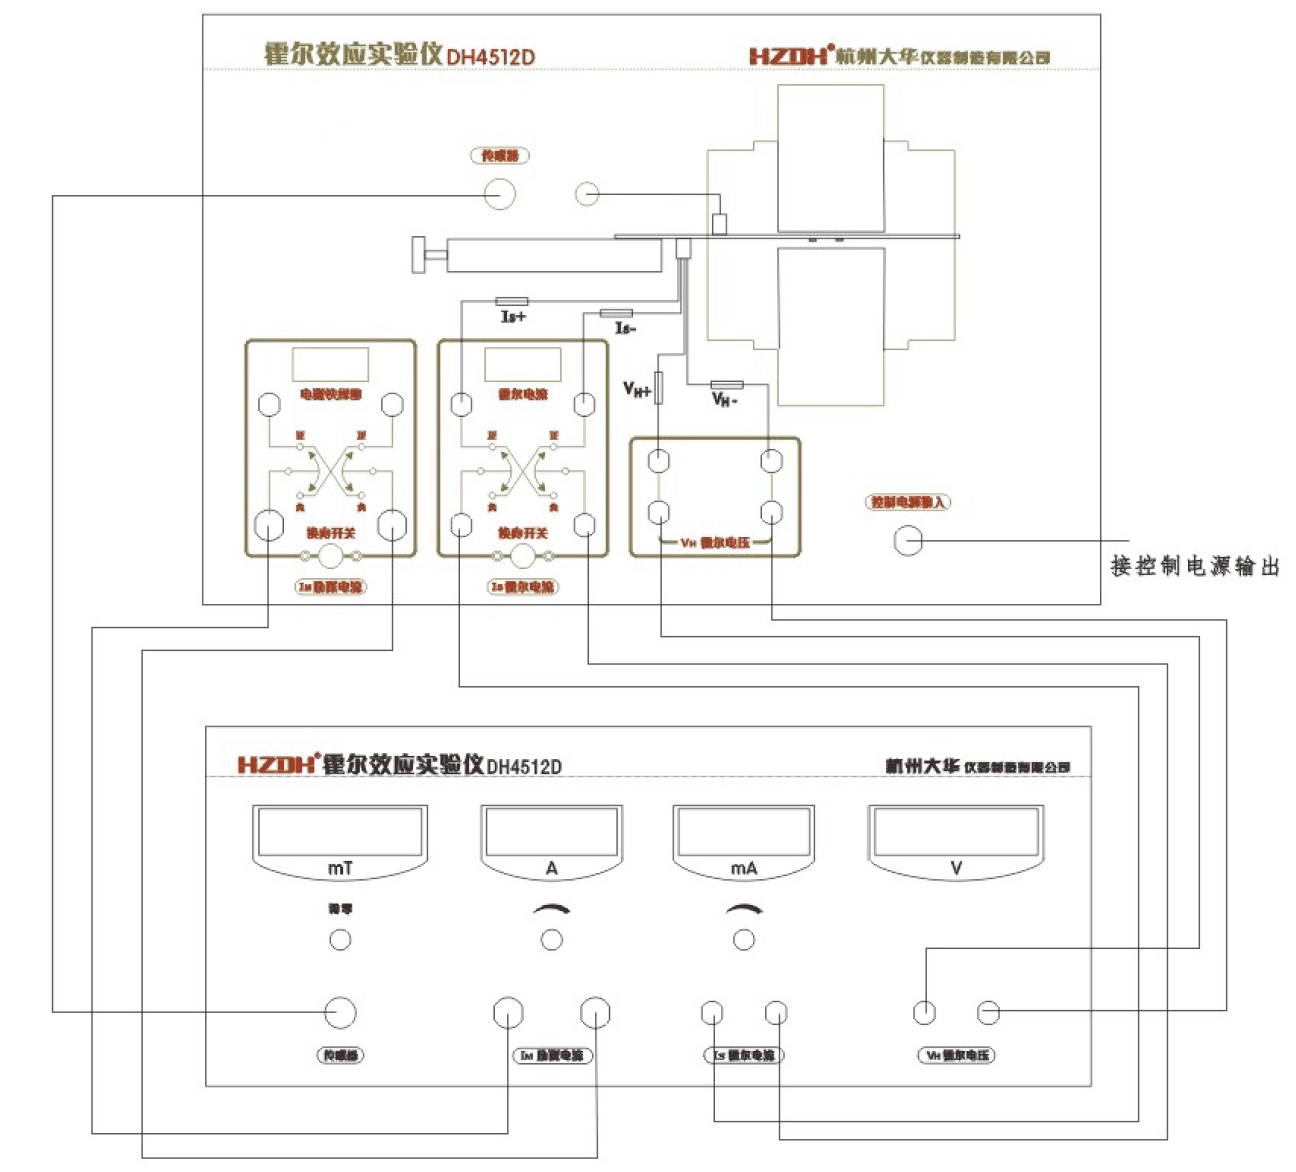
\includegraphics[width=9cm]{Fig/3.png}
        \caption{接线图}
    \end{figure}
    \item 如图连接线材。将霍尔片调整至磁铁中心。将所有旋钮逆时针旋转至最小。
    \item 打开电源,调整$I_M$为0的情况下调整其他数值为0。此调零在下面每个分实验之前都做一次。
    \item 依照表1-表4要求进行测量。
    \item 将$I_S$输入改为用信号发生器产生的正弦交流电流,用万用表串联进电路测$I_S$,改变$I_M$,用台式万用表测量$v_{H-AC}$,用上实验中的仪器测量$B$。
\end{enumerate}

\subsection{实验数据}

\begin{table}[H]
    \centering
    \caption{霍尔电压$V_H$与工作电流$I_S$数据记录($V_H-I_S,\quad I_M=200mA$)}
    \begin{tabular}{|c|c|c|c|c|c|}
    \hline
        \multirow{2}*{$I_S/mA$} & $V_1/mV$ & $V_2/mV$ & $V_3/mV$ & $V_4/mV$ & \multirow{2}*{$V_H/mV$} \\ 
              & $+I_M\quad +I_S$ & $+I_M\quad -I_S$ & $-I_M\quad -I_S$ & $-I_M\quad +I_S$ & ~  \\ \hline
        0 & 0 & 0 & 0 & 0 & 0 \\ \hline
        0.50  & 23.8  & -24.1  & -23.8  & 24.0  & 23.9 \\ \hline
        1.00  & 48.2  & -48.1  & -47.8  & 48.4  & 48.1 \\ \hline
        1.50  & 72.3  & -72.5  & -71.8  & 72.2  & 72.2 \\ \hline
        2.00  & 93.8  & -95.6  & -94.8  & 95.9  & 95.0 \\ \hline
        2.50  & 120.3  & -119.2  & -118.3  & 120.0  & 119.4 \\ \hline
        3.00  & 143.8  & -143.6  & -142.4  & 145.3  & 143.8 \\ \hline
    \end{tabular}
    \label{tab:1}
\end{table}
\begin{table}[H]
    \centering
    \caption{霍尔电压$V_H$与励磁电流$I_M$数据记录($V_H-I_M,\quad I_S=1.00mA$)}
    \begin{tabular}{|c|c|c|c|c|c|}
    \hline
    \multirow{2}*{$I_M/mA$} & $V_1/mV$ & $V_2/mV$ & $V_3/mV$ & $V_4/mV$ & \multirow{2}*{$V_H/mV$} \\ 
    & $+I_M\quad +I_S$ & $+I_M\quad -I_S$ & $-I_M\quad -I_S$ & $-I_M\quad +I_S$ & ~  \\ \hline
        0  & 0 & 0 & 0 & 0 & 0 \\ \hline
        50  & 8.8 & -8.6 & -8.7 & 8.8 & 8.7 \\ \hline
        100  & 21.7 & -21.6 & -21.6 & 21.8 & 21.7 \\ \hline
        150  & 34.8 & -34.7 & -34.7 & 34.8 & 34.8 \\ \hline
        200  & 47.8 & -47.5 & -47.4 & 48.1 & 47.7 \\ \hline
        250  & 60.8 & -60.4 & -60.7 & 60.8 & 60.7 \\ \hline
        300  & 73.4 & -73.4 & -73.2 & 73.5 & 73.4 \\ \hline
    \end{tabular}
    \label{tab:2}
\end{table}
\begin{table}[H]
    \centering
    \caption{磁感应强度$B$与励磁电流$I_M$数据记录($B-I_M,\quad I_S=1.00mA$)}
    \begin{tabular}{|c|c|c|c|c|c|}
    \hline
    \multirow{2}*{$I_M/mA$} & $B_1/mT$ & $B_2/mT$ & $B_3/mT$ & $B_4/mT$ & \multirow{2}*{$B/mT$} \\ 
    & $+I_M\quad +I_S$ & $+I_M\quad -I_S$ & $-I_M\quad -I_S$ & $-I_M\quad +I_S$ & ~  \\ \hline
        0  & 0.0  & 0.0  & 0.0  & 0.0  & 0.0  \\ \hline
        50  & 35.3  & 35.3  & 35.3  & 35.3  & 35.3  \\ \hline
        100  & 71.0  & 71.0  & 71.1  & 71.1  & 71.0  \\ \hline
        150  & 106.8  & 106.9  & 107.4  & 107.6  & 107.2  \\ \hline
        200  & 143.1  & 143.2  & 142.4  & 143.9  & 143.2  \\ \hline
        250  & 178.8  & 178.1  & 179.0  & 178.9  & 178.7  \\ \hline
        300  & 213.8  & 213.8  & 213.9  & 213.8  & 213.8 \\ \hline
    \end{tabular}
    \label{tab:3}
\end{table}
\begin{table}[H]
    \centering
    \caption{电磁铁磁场沿水平方向分布数据记录图($I_M=200mA$)}
    \begin{tabular}{|c|c|c|c|c|c|c|c|c|}
    \hline
        $X/mm$ & 44 & 42 & 40 & 38 & 36 & 34 & 32 & 30 \\ \hline
        $B/mT$ & 36.0  & 59.1  & 112.5  & 140.4  & 142.8  & 142.8  & 142.8  & 143.0  \\ \hline
        $X/mm$ & 28 & 26 & 24 & 22 & 20 & 18 & 16 & 14 \\ \hline
        $B/mT$ & 143.1  & 143.2  & 143.2  & 143.2  & 143.4  & 142.6  & 142.2  & 142.4 \\ \hline
    \end{tabular}
    \label{tab:4}
\end{table}
\begin{table}[H]
    \centering
    \caption{AC模式霍尔效应测量磁场($I_{S-AC}=1mA$)}
    \begin{tabular}{|c|c|c|c|c|}
    \hline
        $I_M/mA$ & 50  & 100  & 150  & 200  \\ \hline
        $B/mT$ & 35.4 & 71.5 & 107 & 144 \\ \hline
        $V_{H-AC}/mV$ & 9.229 & 22.176 & 35.094 & 48.311 \\ \hline
    \end{tabular}
    \label{tab:5}
\end{table}
\subsection{数据处理}
\begin{figure}[H]
    \centering
    \begin{minipage}[t]{0.49\linewidth}
        \centering
        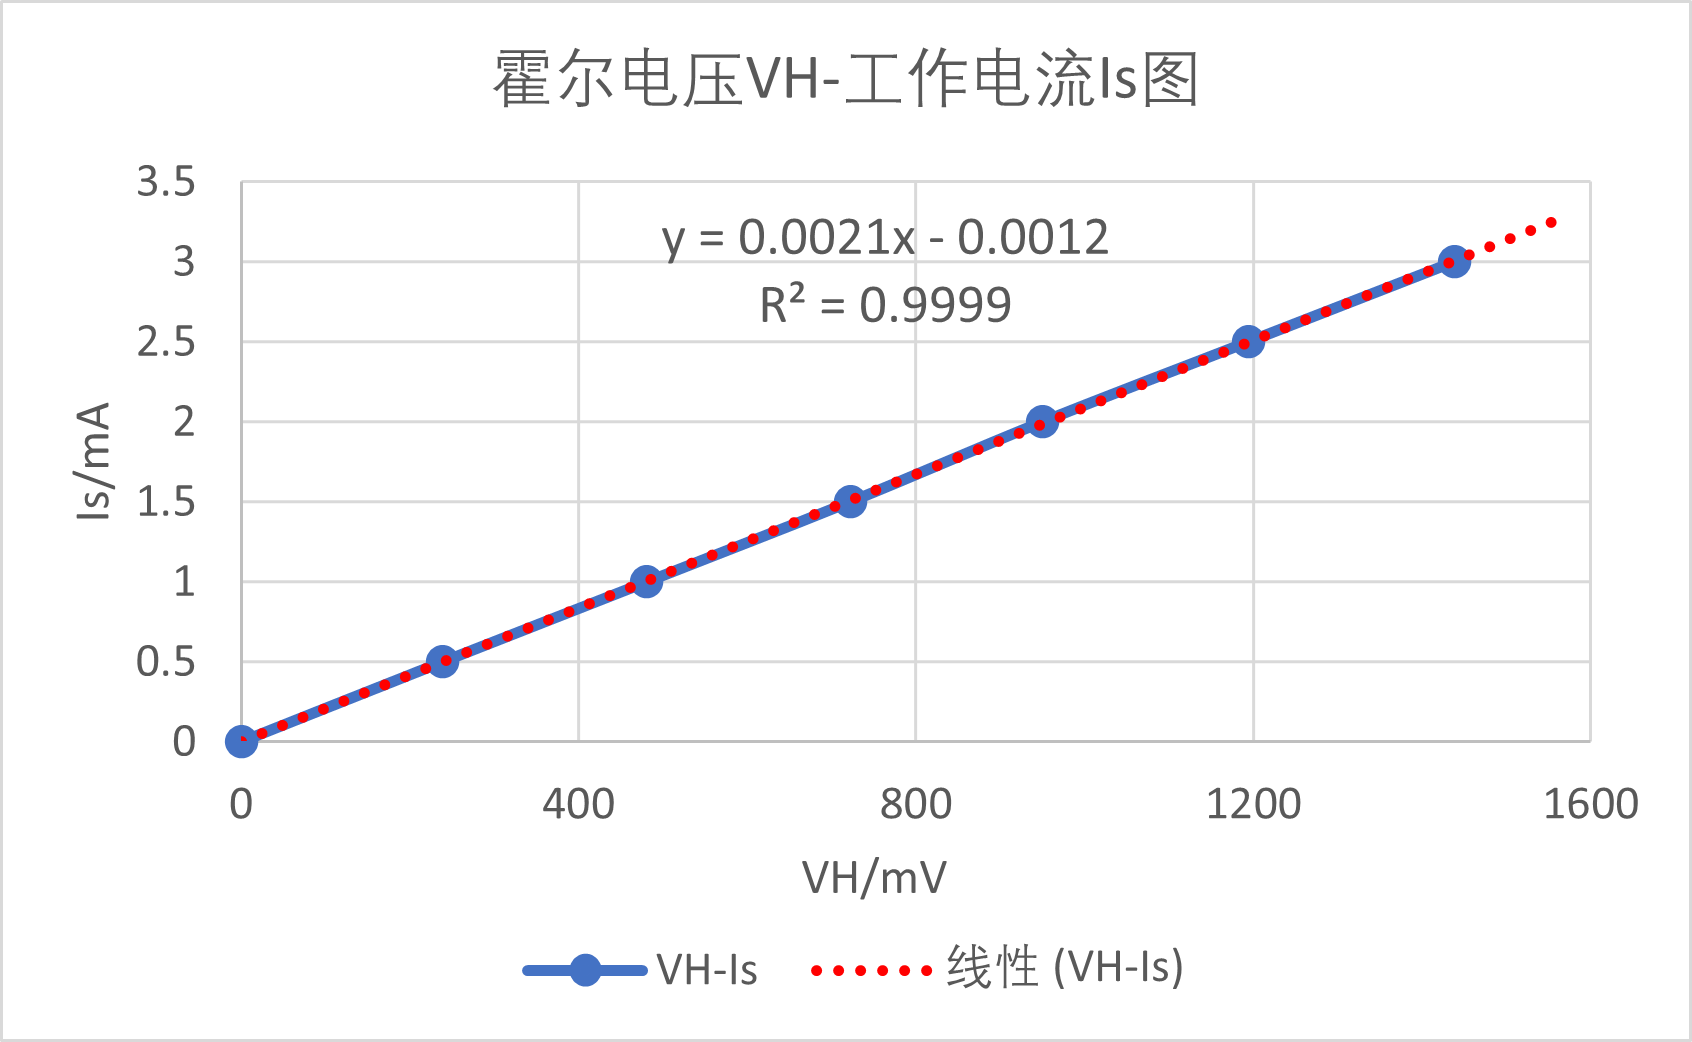
\includegraphics[width=7.8cm]{Fig/4.png}
        \caption{工作电流$I_S$-霍尔电压$V_H$图}
        \label{fig:4}
    \end{minipage}
    \begin{minipage}[t]{0.49\linewidth}
        \centering
        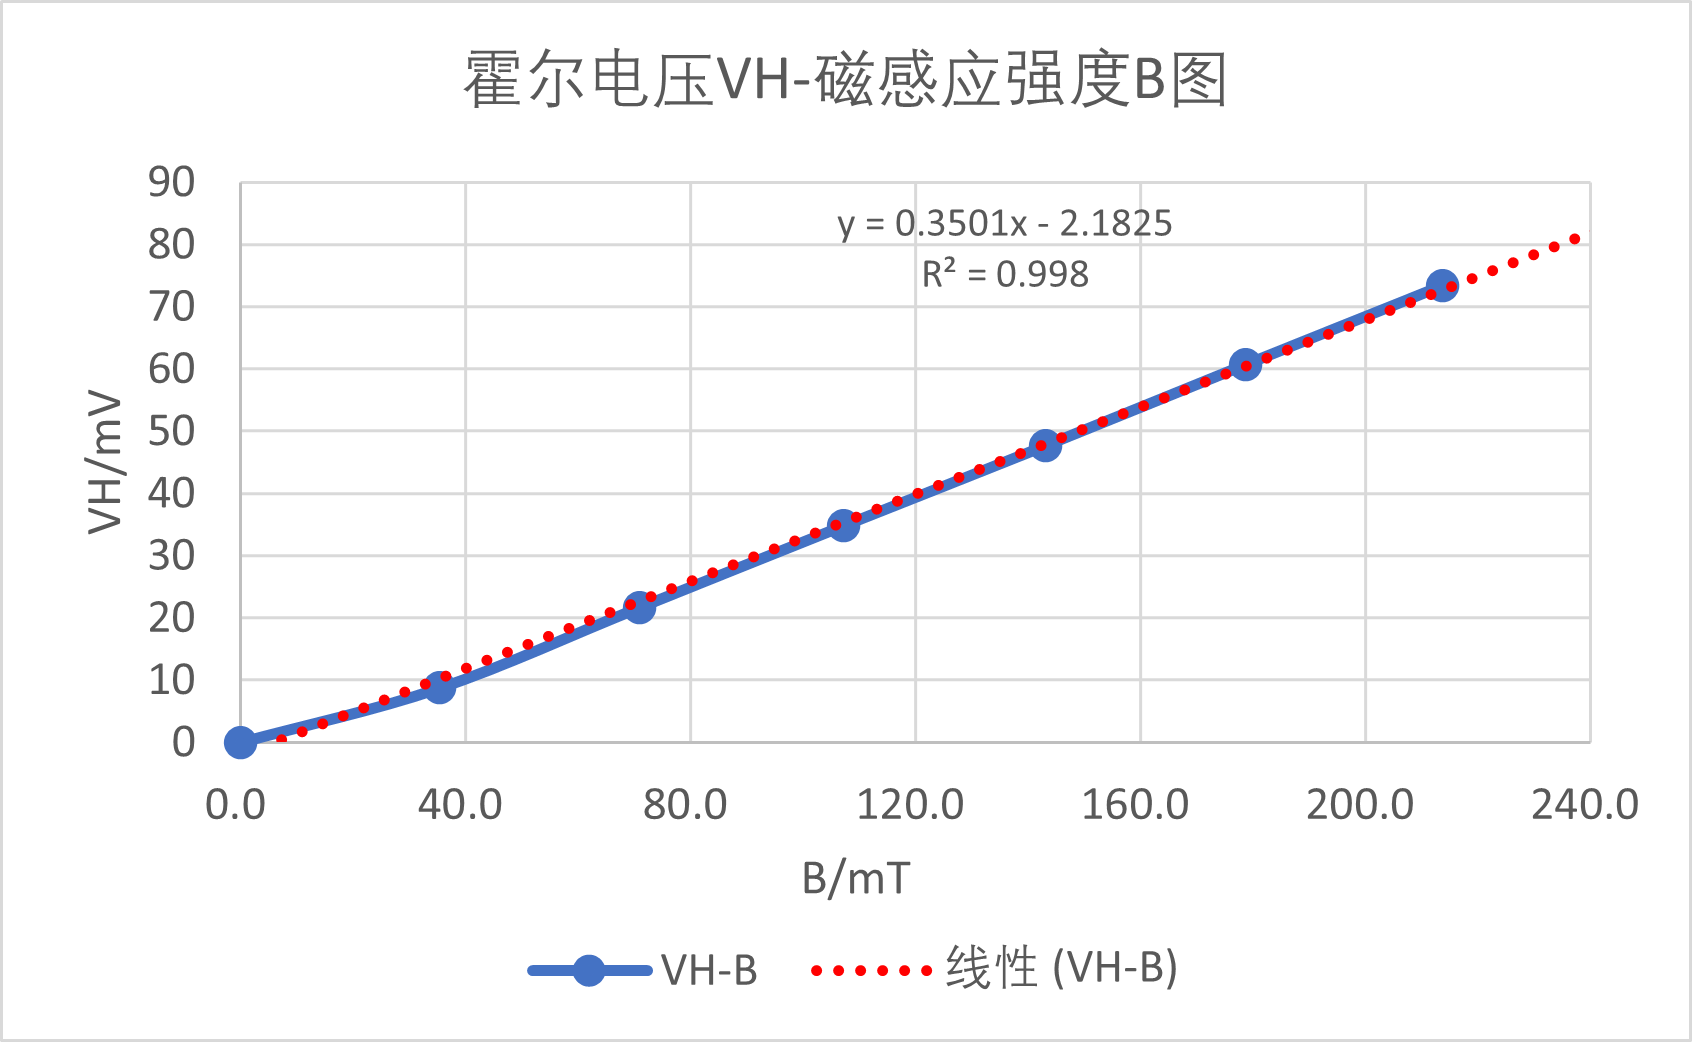
\includegraphics[width=7.8cm]{Fig/5.png}
        \caption{霍尔电压$V_H$-磁感应强度$B$图}
        \label{fig:5}
    \end{minipage}
    
\end{figure}
\par \cref{fig:4}是表\ref{tab:1}数据作图,可以看到拟合结果$V_H=0.0021I_S-0.0012(mV)$,$V_H$与$I_S$有良好的线性关系。
     \cref{fig:5}是表\ref{tab:2}和表\ref{tab:3}数据作图,可以看到拟合结果$V_H=0.3501B-2.1825$,在$V_H$较小时线性较差,整体$V_H$与$B$有良好的线性关系。
\par $K_H=\frac{V_H}{B}\frac{1}{I_S}=350.1(mV/T)/1(mA)=350.1\left[mV/(T*mA)\right]$。实验器材上记录的$K_H=350\left[mV/(T*mA)\right]$,在保留三位有效数字的情况下,测量值与标记值完全相同,无误差。

\begin{figure}[H]
    \centering
    \begin{minipage}[t]{0.49\linewidth}
        \centering
        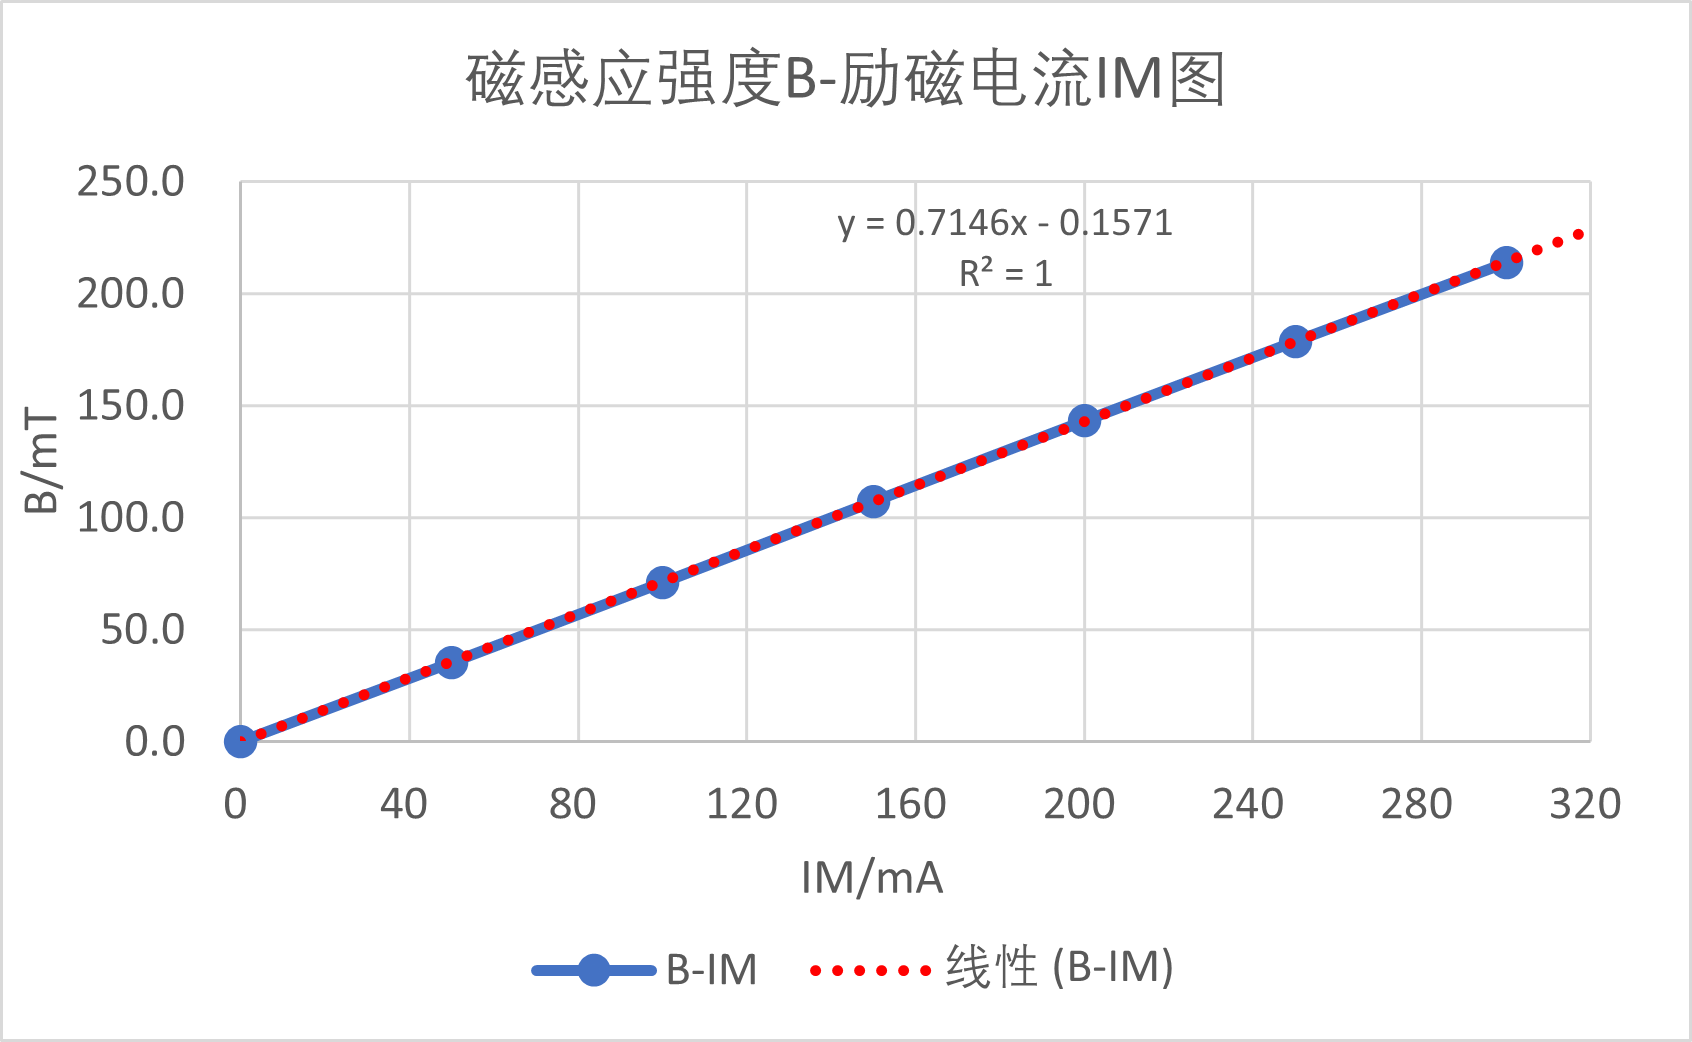
\includegraphics[width=7.8cm]{Fig/6.png}
        \caption{磁感应强度$B$-励磁电流$I_M$图}
        \label{fig:6}
    \end{minipage}
    \begin{minipage}[t]{0.49\linewidth}
        \centering
        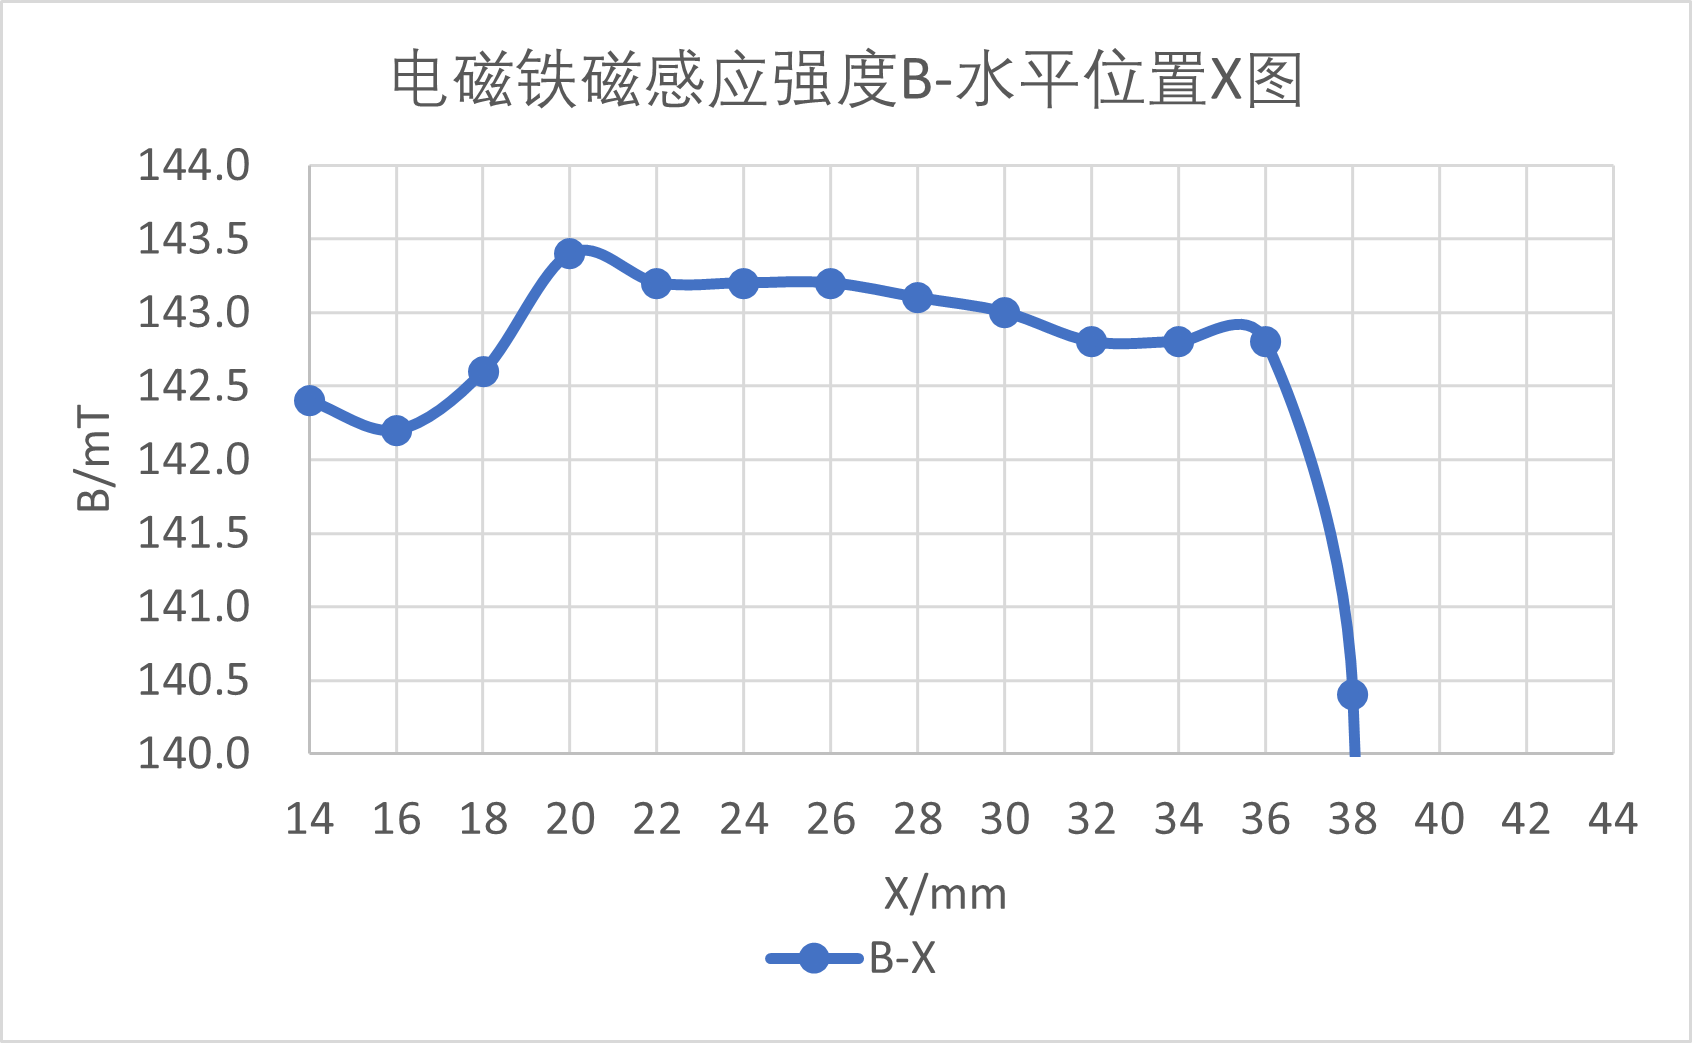
\includegraphics[width=7.8cm]{Fig/7.png}
        \caption{电磁铁磁感应强度B-水平位置X图}
        \label{fig:7}
    \end{minipage}
\end{figure}    
\par \cref{fig:6}是表\ref{tab:3}数据作图,可以看到拟合结果$B=0.7146I_M-0.1571(mT)$,$B$与$I_M$有良好的线性关系。同时,$R^2$在保留小数点后四位的情况下为1.0000,说明磁感应强度由励磁电流生成时为线性,几乎无误差。
\par \cref{fig:7}是表\ref{tab:4}数据作图,中间部分$B$应保持最大值,但有部分误差。误差分析在后文叙述。
\begin{figure}[H]
    \centering
    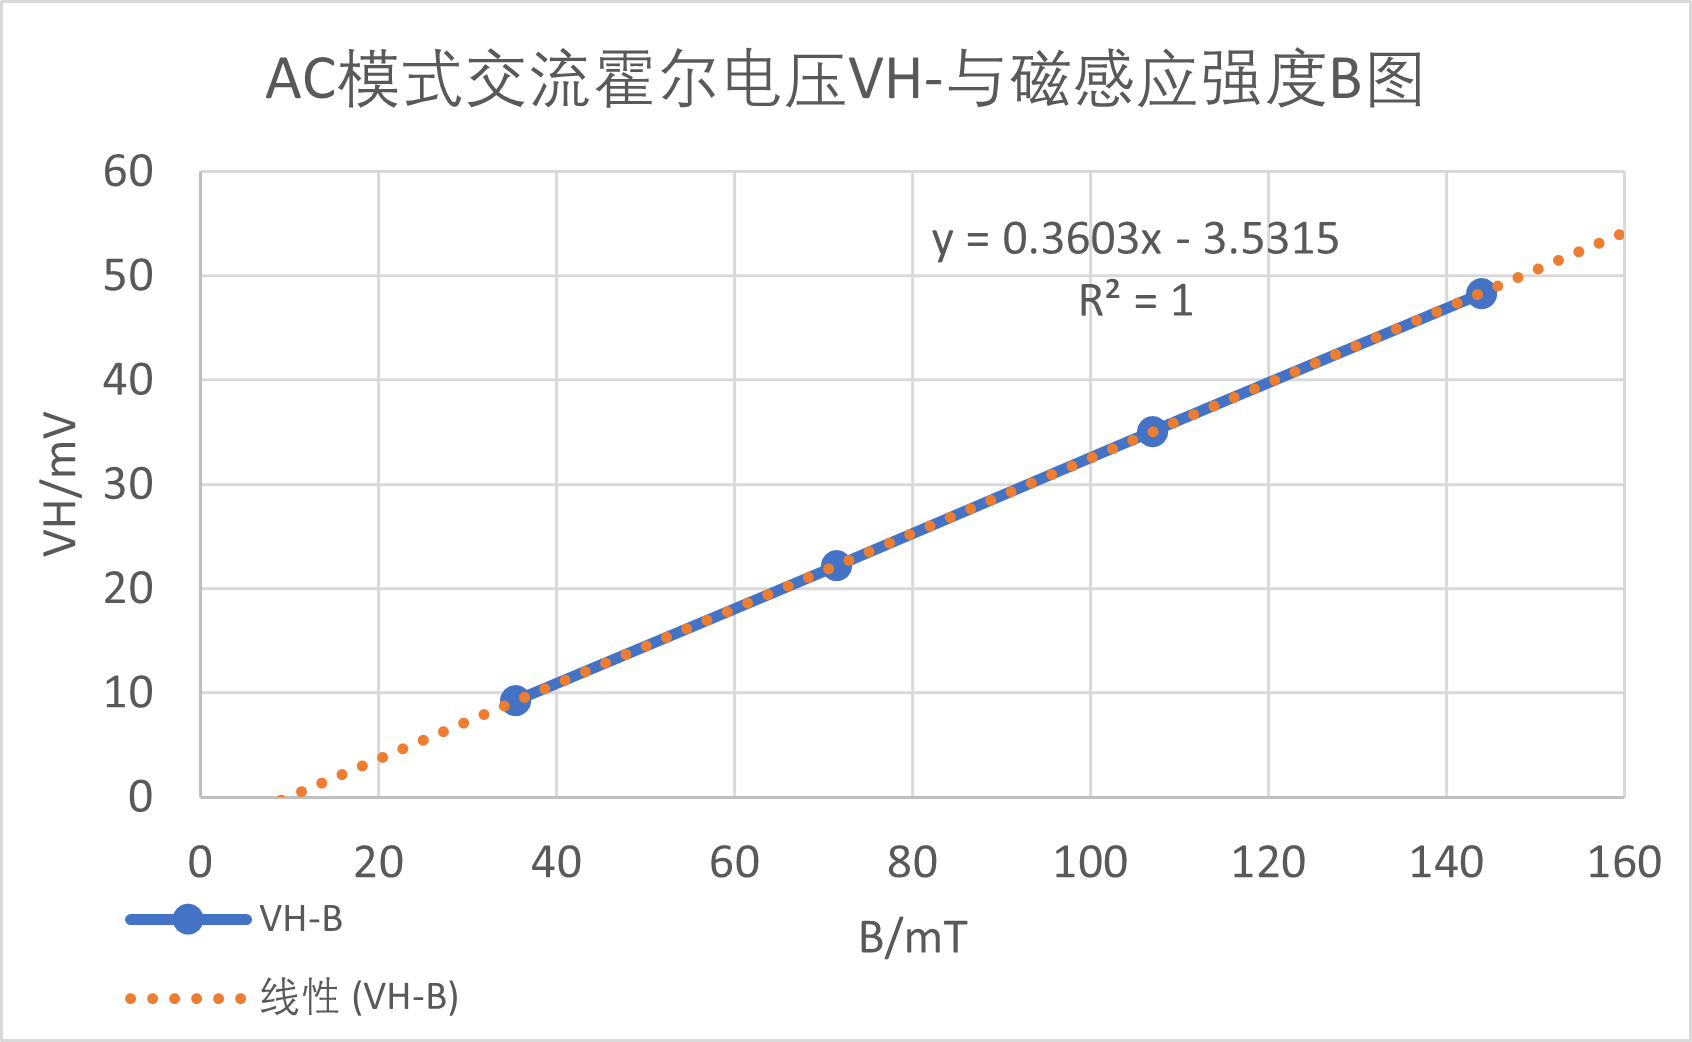
\includegraphics[width=10cm]{Fig/8.png}
    \caption{AC模式交流霍尔电压$V_H$-与磁感应强度B图}
    \label{fig:8}
\end{figure}
\par \cref{fig:8}是表\ref{tab:5}数据作图,拟合结果$V_H=0.3603B-3.5315(mV)$,所计算的$K_H=360.3\left[mV/(T*mA)\right]$,与直流模式测量值有$2.9\%$的误差。但交流模式下的拟合直线$R^2$值比直流时更大,说明交流情况下$V_H$测量误差更小。交流模式所测的电压与电流都为有效值,说明磁场的产生应和励磁电流对应的功率有关。
表\ref{tab:5}测量与直流测量的误差:磁感应强度B最大误差$\frac{71.5-71.0}{71.0}=0.7\%$,霍尔电压最大误差$V_H=\frac{9.229-8.7}{9.229}=5.7\%$。
\subsection{误差分析}

\begin{enumerate}
    \item 造成上面实验拟合图像截距不为0的原因:B调零时的误差,$V_H$测量误差导致的拟合图像误差。
    \begin{figure}[!ht]
        \centering
        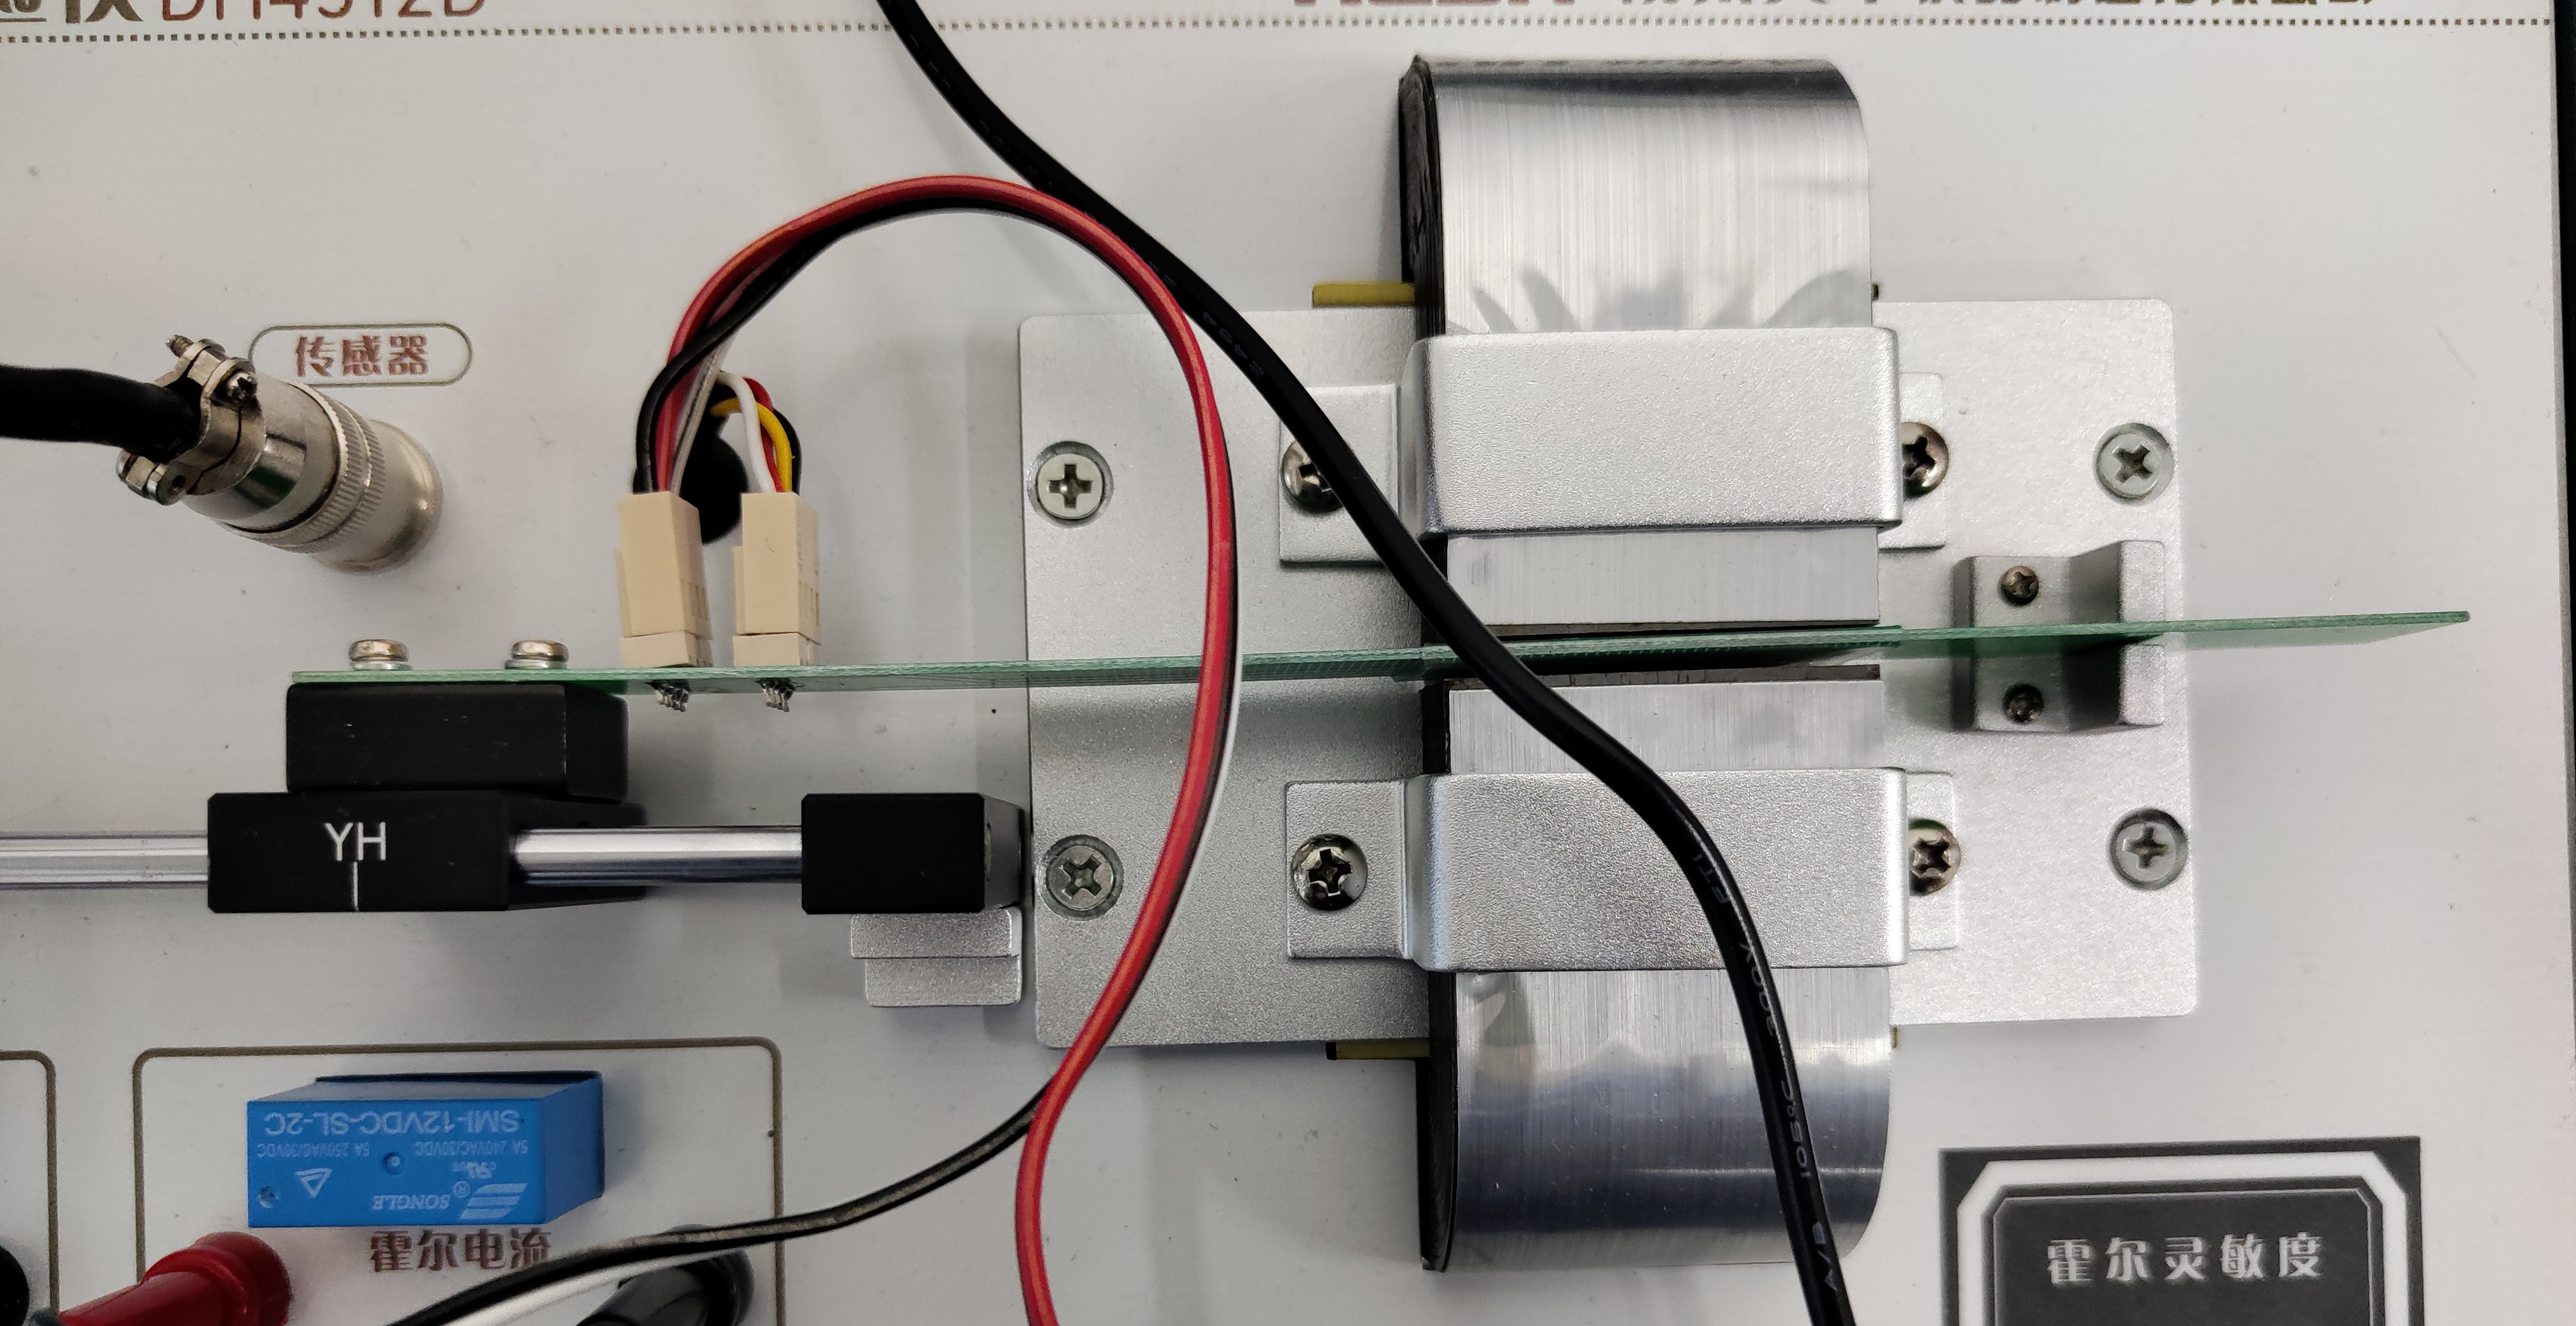
\includegraphics[width=10cm]{Fig/9.jpg}
        \caption{霍尔片与磁铁位置}
        \label{fig:9}
    \end{figure}
    \item 造成\cref{fig:7}中间部分$B$最大值不恒定的原因:电磁场与霍尔片不垂直(如\cref{fig:9}),输入电流微小波动,实验操作问题。当$\theta=2.5^\circ$时,$\cos \theta =0.9990$,当$B=143mT$时会带来$\pm0.14$的误差,小于实验中的误差。实际上,我实验时没有按照刻度条上的刻度进行读数,而是从尺子能移动到的最右端开始读数。读数时取最大值,但读数有波动不稳定,波动的范围大约$\pm 0.3mT$。综合上述因素造成较大的实验误差,导致最大值处数据不平。
    \item 造成表\ref{tab:5}与表\ref{tab:3}表\ref{tab:4}误差的原因:
    \par \hspace*{2em}首先,两实验仪器不同,具有仪器误差。台式万用表的精度高于磁场测量仪自带的电压表。其次,励磁电流较小时,使用对称交换测量法时由于测量的$V_1$-$V_4$较小,测量误差占比较大,因此误差较大,而交流法不涉及此问题。
\end{enumerate}
\subsection{思考题}
\begin{enumerate}
    \item 分析本实验主要误差来源,计算磁感应强度$B$的合成不确定度(分别取$I_M=0.2A$,$I_S=1mA$)。
    \par \hspace*{2em}表\ref{tab:3}:数字式特斯拉计测量范围0-1000mT,最小分辨率0.1mT。磁感应强度测量不确定度$u_b(B)=0.1mT$。
    励磁电流$I_M$可调范围0-0.5A,调节细度<1mA,励磁电流测量误差$u_B(I_M)=1mA$。
    霍尔工作电流$I_S$可调范围0-3.5mA,最小分辨率0.01mA,$I_S$测量不确定度$0.01$。
    由
    \[u(B)=B_{max}\sqrt{\frac{{U_B(B)}^2}{B^2}+\frac{{u_b(I_M)}^2}{{I_M}^2}+\frac{{u_b(I_S)}^2}{{I_S}^2}}=2.4mT\]
    偏差率$\frac{u(B)}{B}=1.1\%$。其中数字式特斯拉计的误差贡献几乎为0。
    \item 以简图示意,用霍尔效应法判断霍尔片上磁感应强度方向。
    \par \hspace*{2em}对N型半导体(电子型),用左手定则,用四指指向电流方向,大拇指与手掌垂直指向电势为负的一面,则磁感应强度方向扎手心而出。
    \par \hspace*{2em}对P型半导体(空穴型),用左手定则,用四指指向电流方向,大拇指与手掌垂直指向电势为正的一面,则磁感应强度方向扎手心而出。
    \item 如何测量交变磁感应强度,写出主要步骤。
    \par \hspace*{2em}由公式\eqref{equ:2.5},测量V_H极大值,计算得B极大值,除以$\sqrt{2}$得有效值。
\end{enumerate}

\begin{center}
    \vspace*{1em}
    \Large \bf 第二部分\qquad 亥姆霍兹线圈的磁感应强度测量
\end{center}
\setcounter{section}{0}
\section{实验目的}
\begin{enumerate}
    \item 掌握载流圆线圈的磁感应强度分布;
    \item 复习并掌握亥姆霍兹线圈的磁感应强度在轴线上的分布和轴线附近的分布。
\end{enumerate}

\section{实验仪器}
    \par 杭州大华DH4501亥姆霍兹磁感应强度实验仪。

\section{实验原理}
\begin{enumerate}
    \item 载流圆线圈的磁感应强度分布
    \par \hspace*{2em}如图\cref{fig:10}一半径为$R$,通以电流$I$的圆线圈,线圈匝数$N_0$,真空磁导率$\mu_0=4\pi\times 10^{-7}(H/m)$,$X$为轴上某一点到圆心O的距离。轴线上磁感应强度的公式为:
    \begin{equation}{\label{equ:6}}
        B=\frac{\mu_0 N_0}{2}\frac{R^2}{\left(R^2+x^2\right)^{3/2}}I
    \end{equation}

    \begin{figure}[!ht]
        \centering
        \begin{minipage}[t]{0.49\linewidth}
            \centering
            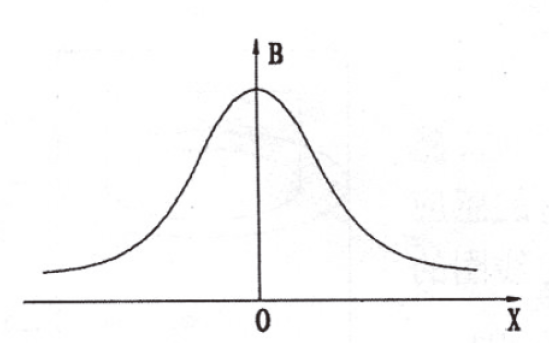
\includegraphics[width=7cm]{Fig/10.png}
            \caption{载流圆线圈轴线上磁感应强度分布}
            \label{fig:10}
        \end{minipage}
        \begin{minipage}[t]{0.49\linewidth}
            \centering
            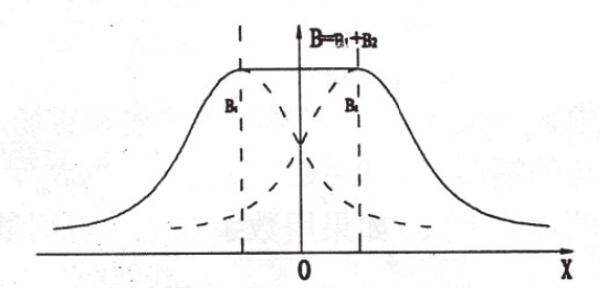
\includegraphics[width=7cm]{Fig/11.png}
            \caption{亥姆霍兹线圈轴线上磁感应强度分布}
            \label{fig:11}
        \end{minipage}
    \end{figure} 

    \item 亥姆霍兹线圈的磁感应强度分布
    \par \hspace*{2em }亥姆霍兹线圈为两个相同线圈彼此平行且共轴,使线圈上通以相同方向电流I,理论计算证明:线圈距离a等于线圈半径R时,两个单个线圈的磁感应强度叠加在轴上(两个线圈的圆心连线)附近较大范围内的合磁感应强度是均匀的,如\cref{fig:11}所示。
    \par \hspace*{2em }设Z为亥姆霍兹线圈中轴线上某一点离中心点O处的距离,则亥姆霍兹线圈轴线上该点的磁感应强度为:
    \begin{equation}
        B=\frac{1}{2}\mu_0 NIR^2\left\{{\left[R^2+\left(\frac{R}{2}+Z\right)^2\right]}^{-\frac{3}{2}}+{\left[R^2+\left(\frac{R}{2}-Z\right)^2\right]}^{-\frac{3}{2}}\right\}
    \end{equation}
    而在亥姆霍兹线圈轴线上中心O处,Z=0,磁感应强度为
    \begin{equation}
        B=\frac{\mu_0 N_0 I}{2R}\frac{16}{5^{3/2}}
    \end{equation}

    \item 电磁感应法测磁感应强度
    \par \hspace*{2em}设磁感应强度最大值$B_m$,角速度$\omega$,则交变磁感应强度有效值$B=B_m \sin \omega t$;磁场中一探测线圈的磁通量$\phi=NSB\cos \theta=NSB_m\cos(\theta) \sin(\omega t)$,其中$N$为探测线圈的匝数,$S$为该线圈的截面积,$\theta$为$B$与线圈法线夹角;线圈产生的磁电动势
    \begin{equation}
        \epsilon=-\frac{d\phi}{dt}=-NS\omega B_m\cos(\theta)\cos(\omega t)=-\epsilon_m \cos(\omega t)
    \end{equation}
    其中$\epsilon_m=NS\omega B_m$,为线圈的最大磁电动势。如果用数字式毫伏表测量此时线圈的电动势,
    则毫伏表的示值(有效值)$U_{max}=\frac{\epsilon_m}{\sqrt{2}}$。则由
    \begin{equation}{\label{equ:10}}
        B_m=\frac{\epsilon_{max}}{NS\omega}=\frac{\sqrt{2}U_{max}}{NS\omega}
    \end{equation}
    可计算出$B_m$。
\end{enumerate}
\section{实验内容}
\subsection{实验步骤}
\begin{enumerate}
    \item 开启实验仪,预热10分钟。
    \item 连接“感应电压”与“输出电压”,按实验需求连接“励磁电流”和“励磁线圈”。
    \item 按照实验表格所需,慢慢转动x轴或y轴手轮,记录数据。
\end{enumerate}
\subsection{实验数据}
\par 整个实验中
\[f=120Hz\text{(除了表 \ref{tab:10})}\qquad I=60mA \qquad N_0=400 \qquad R=105mm\]
由公式\eqref{equ:10},$B\text{测量}=\frac{2.923}{f}U_{max}$,我所计算得出的系数是2.923,与表格中给出的系数2.926略有不同。每个$B\text{测量}$后均注明系数。
\\由公式\eqref{equ:6},表\ref{tab:6}中的$B\text{计算}=1.663\times 10^{-4}(R^2+X^2)^{-3/2}$。
\\表\ref{tab:9}中计算值$U'=U_{max}\cdot \cos\theta$。
\begin{table}[H]
    \centering
    \caption{圆电流线圈轴线上磁场分布测量数据记录}
    \begin{tabular}{|c|c|c|c|c|c|c|c|c|c|c|c|}
    \hline
        $X/mm$ & -25 & -20 & -15 & -10 & -5 & 0 & 5 & 10 & 15 & 20 & 25 \\ \hline
        $U_{max}/mV$ & 5.58  & 5.75  & 5.90  & 6.01  & 6.08  & 6.11  & 6.09  & 6.04  & 5.94  & 5.81  & 5.64  \\ \hline
        $B\text{测量}(2.923)/mT$ & 0.136  & 0.140  & 0.144  & 0.146  & 0.148  & 0.149  & 0.148  & 0.147  & 0.145  & 0.142  & 0.137  \\ \hline
        $B\text{计算}/mT$ & 0.132  & 0.136  & 0.139  & 0.142  & 0.143  & 0.144  & 0.143  & 0.142  & 0.139  & 0.136  & 0.132  \\ \hline
        $B\text{测量}(2.827)/mT$ & 0.131  & 0.135  & 0.139  & 0.142  & 0.143  & 0.144  & 0.143  & 0.142  & 0.140  & 0.137  & 0.133 \\ \hline
    \end{tabular}
    \label{tab:6}
\end{table}

\begin{table}[H]
    \centering
    \caption{亥姆霍兹线圈磁场径向分布测量数据记录}
    \begin{tabular}{|c|c|c|c|c|c|c|}
    \hline
        $X/mm$ & -25 & -20 & -15 & -10 & -5 & 0 \\ \hline
        $U_{max}/mV$ & 8.66  & 8.69  & 8.70  & 8.71  & 8.71  & 8.70  \\ \hline
        $B\text{测量}(2.923)/mT$ & 0.211  & 0.212  & 0.212  & 0.212  & 0.212  & 0.212 \\ \hline
        $X/mm$ & 5 & 10 & 15 & 20 & 25 & ~ \\ \hline
        $U_{max}/mV$ & 8.70  & 8.70  & 8.70  & 8.70  & 8.69  & ~ \\ \hline
        $B\text{测量}(2.923)/mT$ & 0.212  & 0.212  & 0.212  & 0.212  & 0.212  &  ~\\ \hline
    \end{tabular}
    \label{tab:7}
\end{table}

\begin{table}[H]
    \centering
    \caption{亥姆霍兹线圈磁场径向分布测量数据记录}
    \begin{tabular}{|c|c|c|c|c|c|c|}
    \hline
        $Y/mm$ & -25 & -20 & -15 & -10 & -5 & 0 \\ \hline
        $U_{max}/mV$ & 8.69  & 8.70  & 8.70  & 8.70  & 8.70  & 8.70  \\ \hline
        $B\text{测量}(2.923)/mT$ & 0.212  & 0.212  & 0.212  & 0.212  & 0.212  & 0.212 \\\hline
        $Y/mm$ & 5 & 10 & 15 & 20 & 25 & ~ \\ \hline
        $U_{max}/mV$ & 8.70  & 8.69  & 8.69  & 8.68  & 8.68  & ~ \\ \hline
        $B\text{测量}(2.923)/mT$ & 0.212  & 0.212  & 0.212  & 0.211  & 0.211  &  \\\hline
    \end{tabular}
    \label{tab:8}
\end{table}
\begin{table}[H]
    \centering
    \caption{探测线圈转角与感应电压数据记录}
    \begin{tabular}{|c|c|c|c|c|c|c|c|c|c|c|}
    \hline
        $\theta/^\circ$ & 0 & 10 & 20 & 30 & 40 & 50 & 60 & 70 & 80 & 90 \\ \hline
        $U/mV$ & 8.70  & 8.56  & 8.17  & 7.61  & 6.73  & 5.75  & 4.55  & 3.09  & 1.63  & 0.08  \\ \hline
        计算值$U'/mV$ & 8.70  & 8.43  & 7.68  & 6.59  & 5.16  & 3.70  & 2.28  & 1.06  & 0.28  & 0.00  \\ \hline
        $\theta/^\circ$ & 100 & 110 & 120 & 130 & 140 & 150 & 160 & 170 & 180 & ~ \\ \hline
        $U/mV$ & 1.44  & 2.91  & 4.30  & 5.57  & 6.73  & 7.54  & 8.17  & 8.52  & 8.60  & ~ \\ \hline
        计算值$U'/mV$ & -0.25  & -1.00  & -2.15  & -3.58  & -5.16  & -6.53  & -7.68  & -8.39  & -8.60 &\\ \hline
    \end{tabular}
    \label{tab:9}
\end{table}
\begin{table}[H]
    \centering
    \caption{励磁电流频率对磁场强度的影响}
    \begin{tabular}{|c|c|c|c|c|c|c|c|c|c|c|c|}
    \hline
        $f/Hz$ & 20 & 30 & 40 & 50 & 60 & 70 & 80 & 90 & 100 & 110 & 120 \\ \hline
        $U_{max}/mV$ & 1.47  & 2.18  & 2.88  & 3.58  & 4.28  & 4.99  & 5.71  & 6.43  & 7.15  & 7.87  & 8.60  \\ \hline
        $B\text{测量}(2.923)/mT$ &0.215  & 0.212  & 0.211  & 0.209  & 0.208  & 0.208  & 0.209  & 0.209  & 0.209  & 0.209  & 0.210  \\\hline
    \end{tabular}
    \label{tab:10}
\end{table}

\subsection{数据处理}
\begin{figure}[H]
    \centering
    \begin{minipage}[t]{0.49\linewidth}
        \centering
        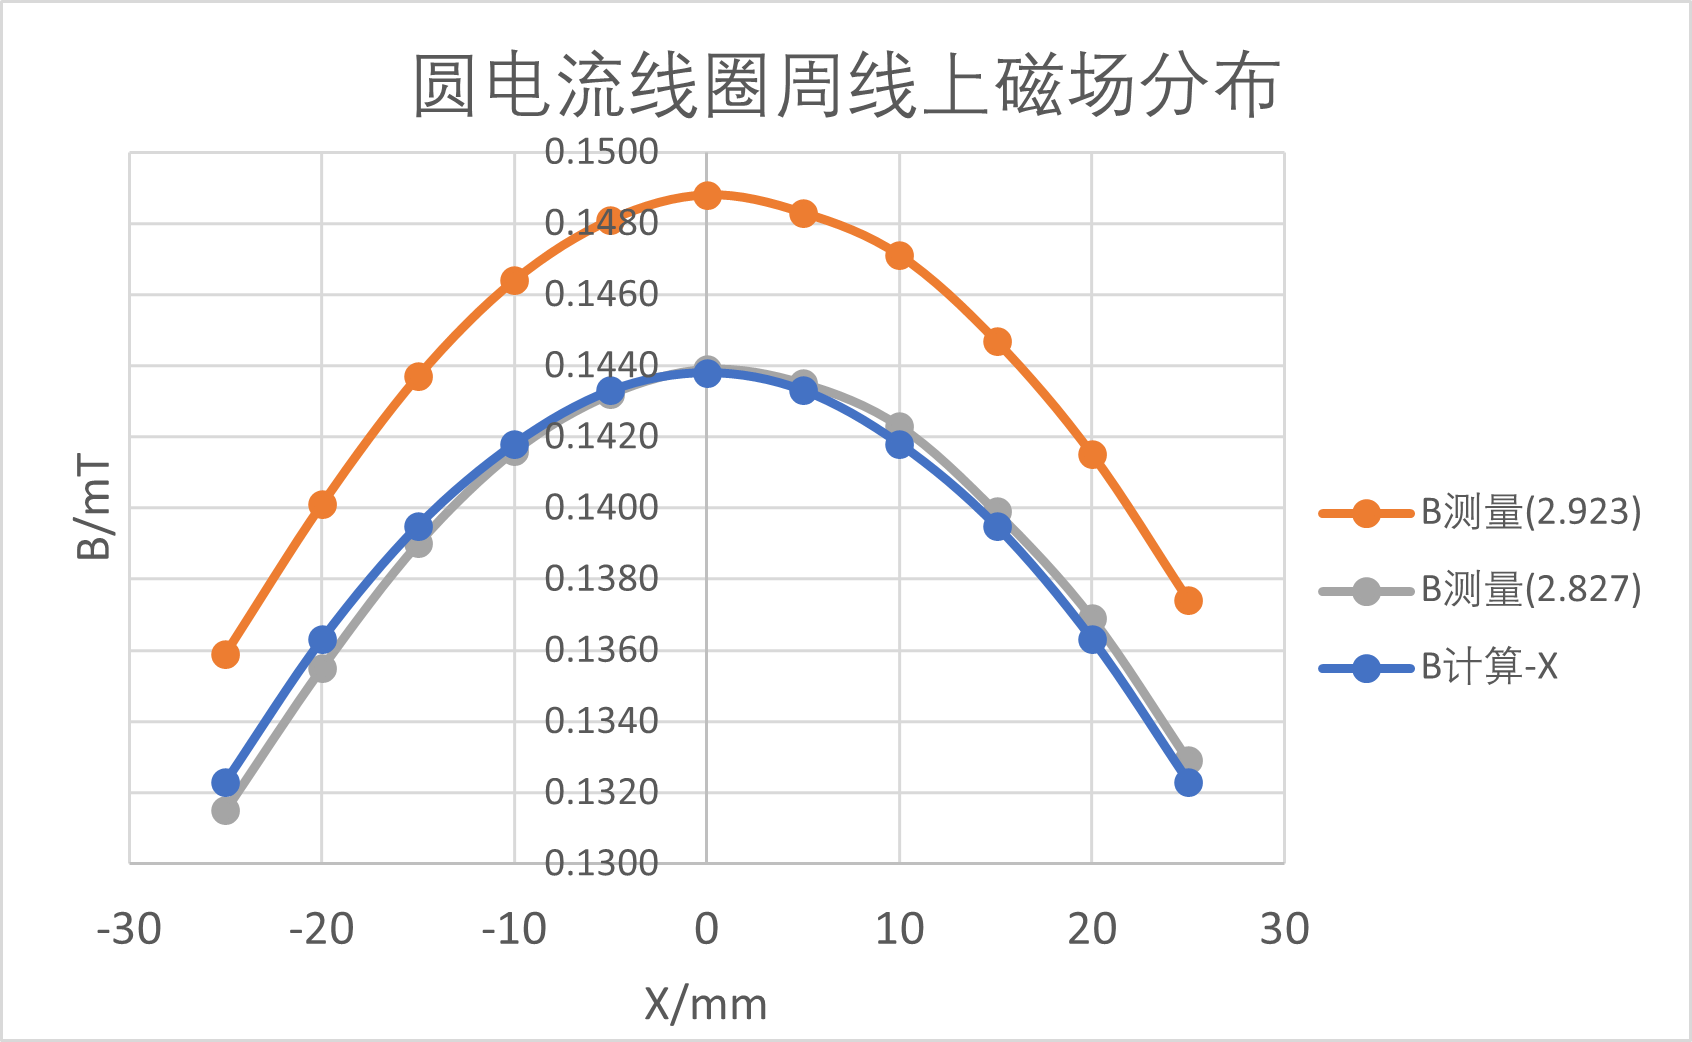
\includegraphics[width=7.8cm]{Fig/12.png}
        \caption{圆电流线圈周线上磁场分布}
        \label{fig:12}
    \end{minipage}
    \begin{minipage}[t]{0.49\linewidth}
        \centering
        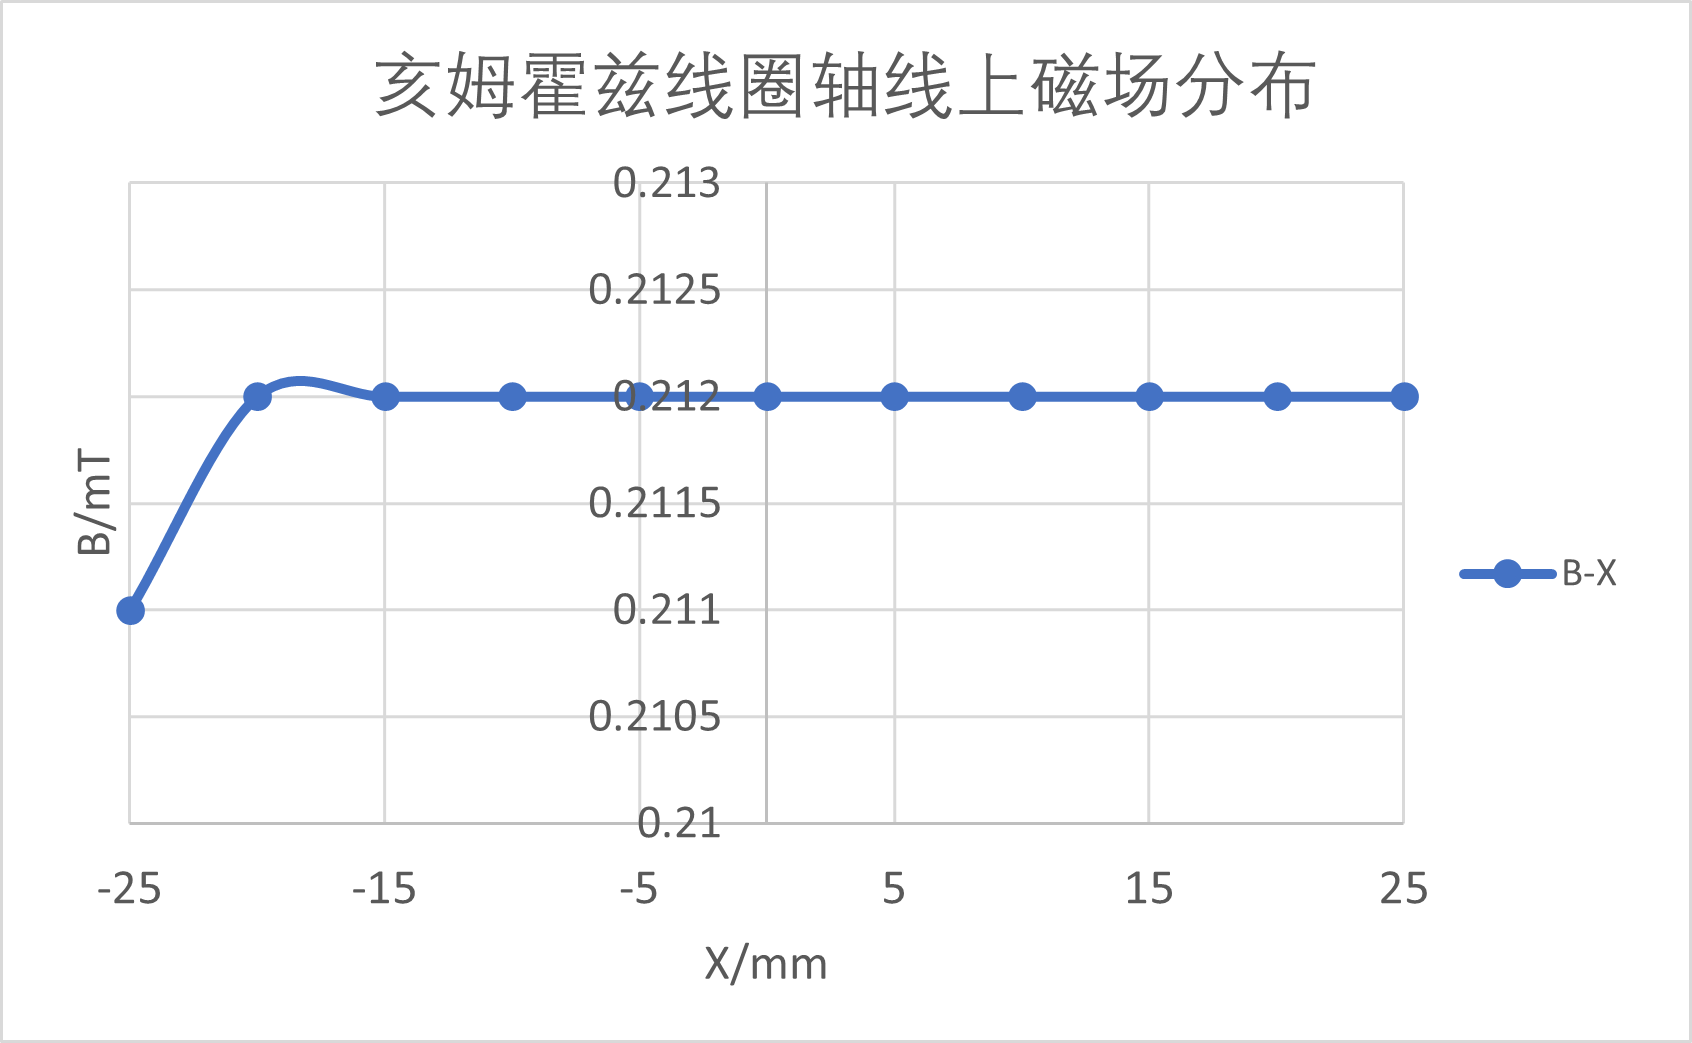
\includegraphics[width=7.8cm]{Fig/13.png}
        \caption{亥姆霍兹线圈轴线上磁场分布}
        \label{fig:13}
    \end{minipage}
\end{figure}
\par \cref{fig:12}是表\ref{tab:6}数据作图,测量值与计算值图形相似。将B测量系数改为2.827后测量值与计算值良好吻合,误差为$1-\frac{2.827}{2.923}=3.3\%$。
\par \cref{fig:13}是表\ref{tab:7}数据作图,可以看到在中间部分磁感应强度都为0.212mT,说明轴向磁场分布均匀。
\begin{figure}[H]
    \centering
    \begin{minipage}[t]{0.49\linewidth}
        \centering
        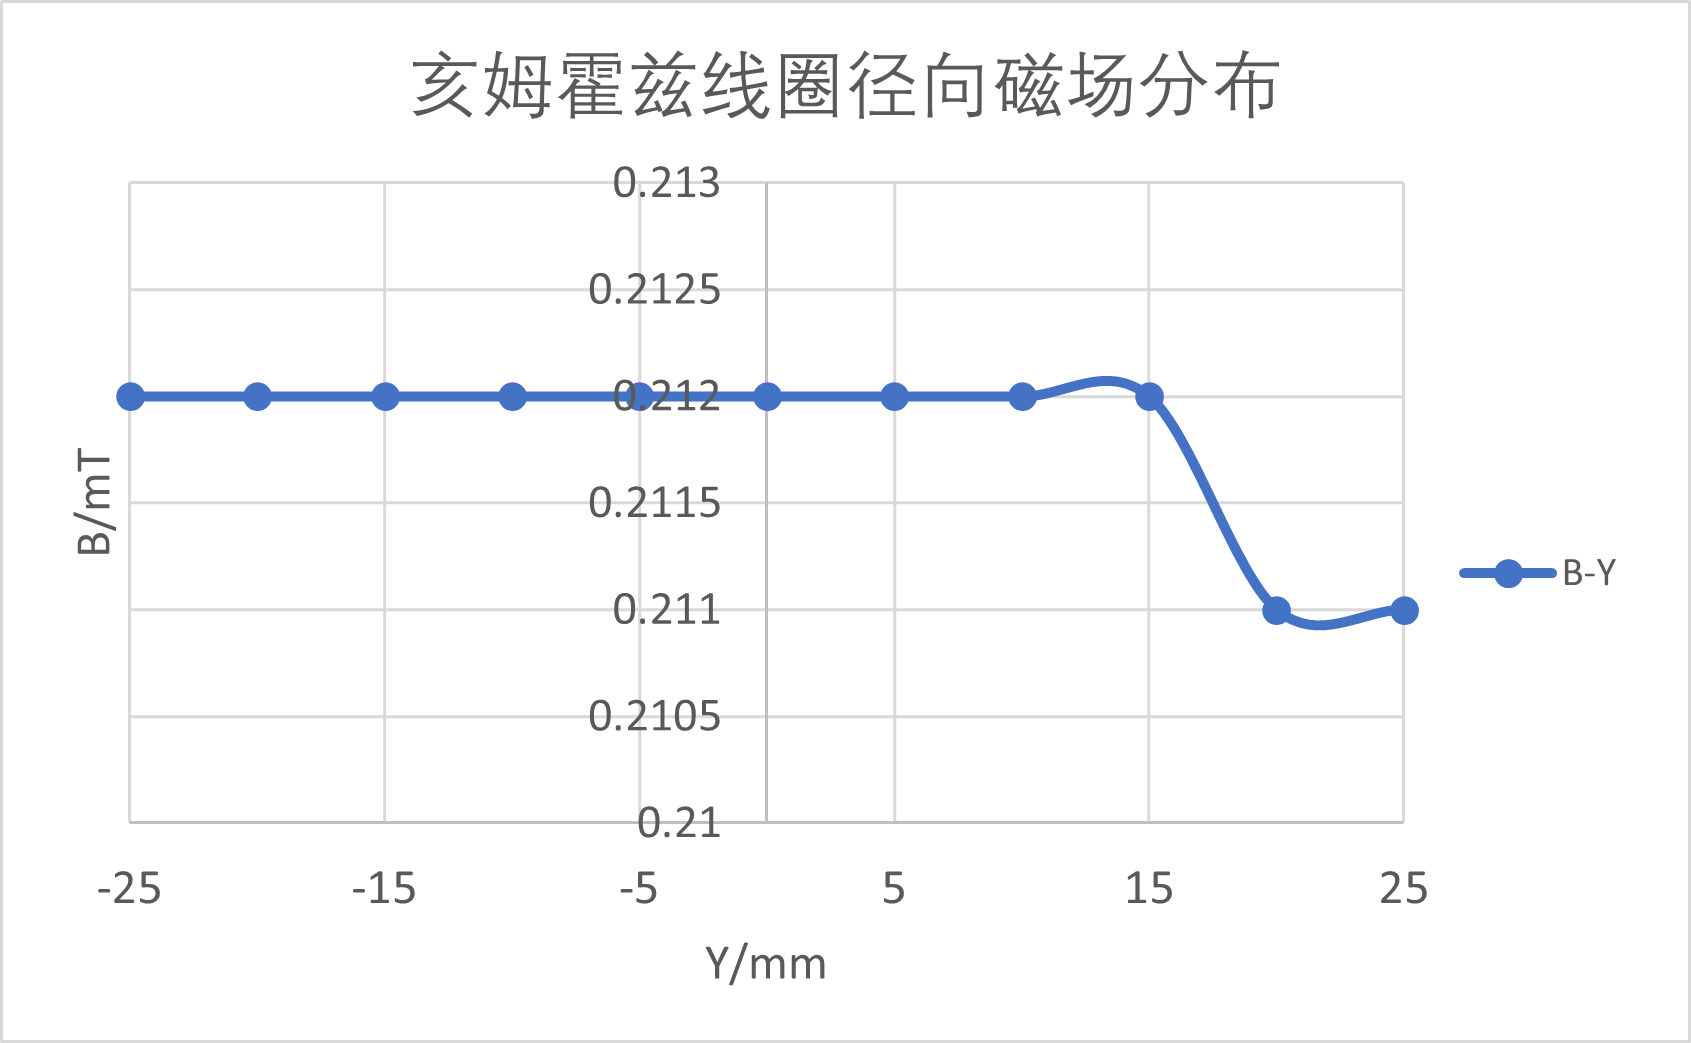
\includegraphics[width=7.8cm]{Fig/14.png}
        \caption{亥姆霍兹线圈径向磁场分布}
        \label{fig:14}
    \end{minipage}
    \begin{minipage}[t]{0.49\linewidth}
        \centering
        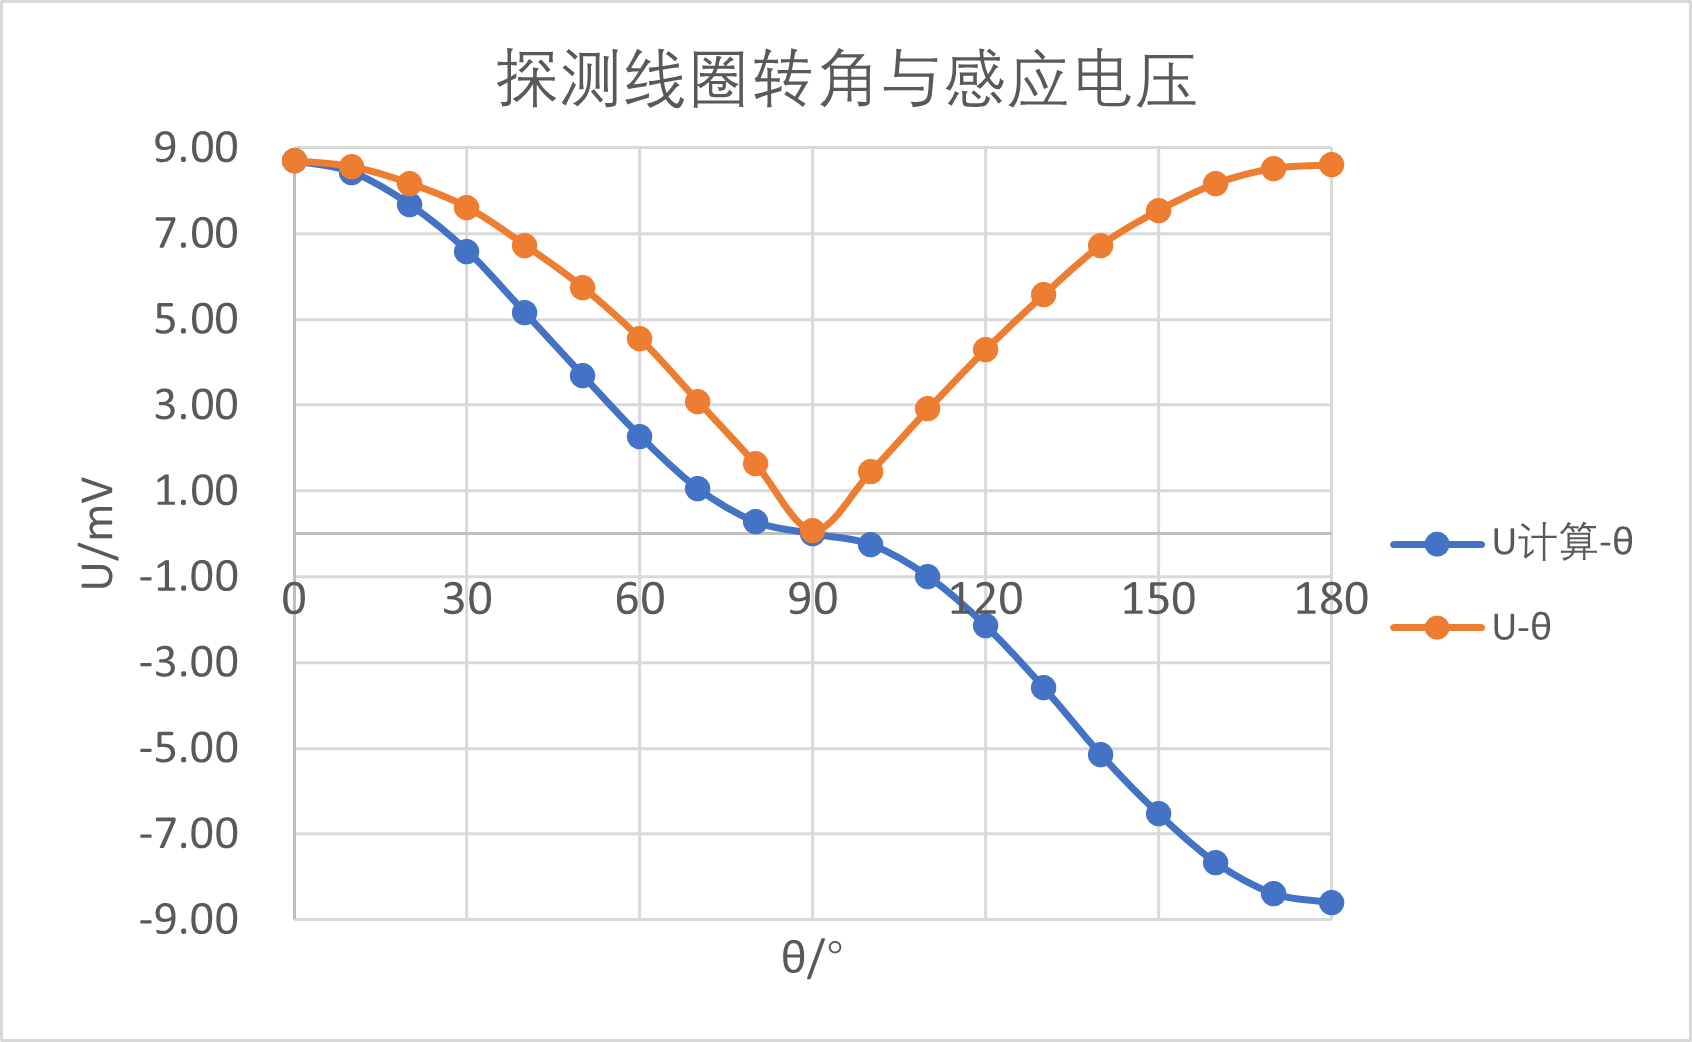
\includegraphics[width=7.8cm]{Fig/15.png}
        \caption{探测线圈转角与感应电压}
        \label{fig:15}
    \end{minipage}
\end{figure}
\par \cref{fig:14}是表\ref{tab:8}数据作图,可以看到在中间部分磁感应强度都为0.212mT,说明径向向磁场分布均匀。
\par \cref{fig:15}是表\ref{tab:9}数据作图,可以看到测量值大致为$\cos$函数,计算值大致为${\cos}^2$函数,说明$\epsilon_m$与$\cos\theta$的线性关系。
\begin{figure}[H]
    \centering
    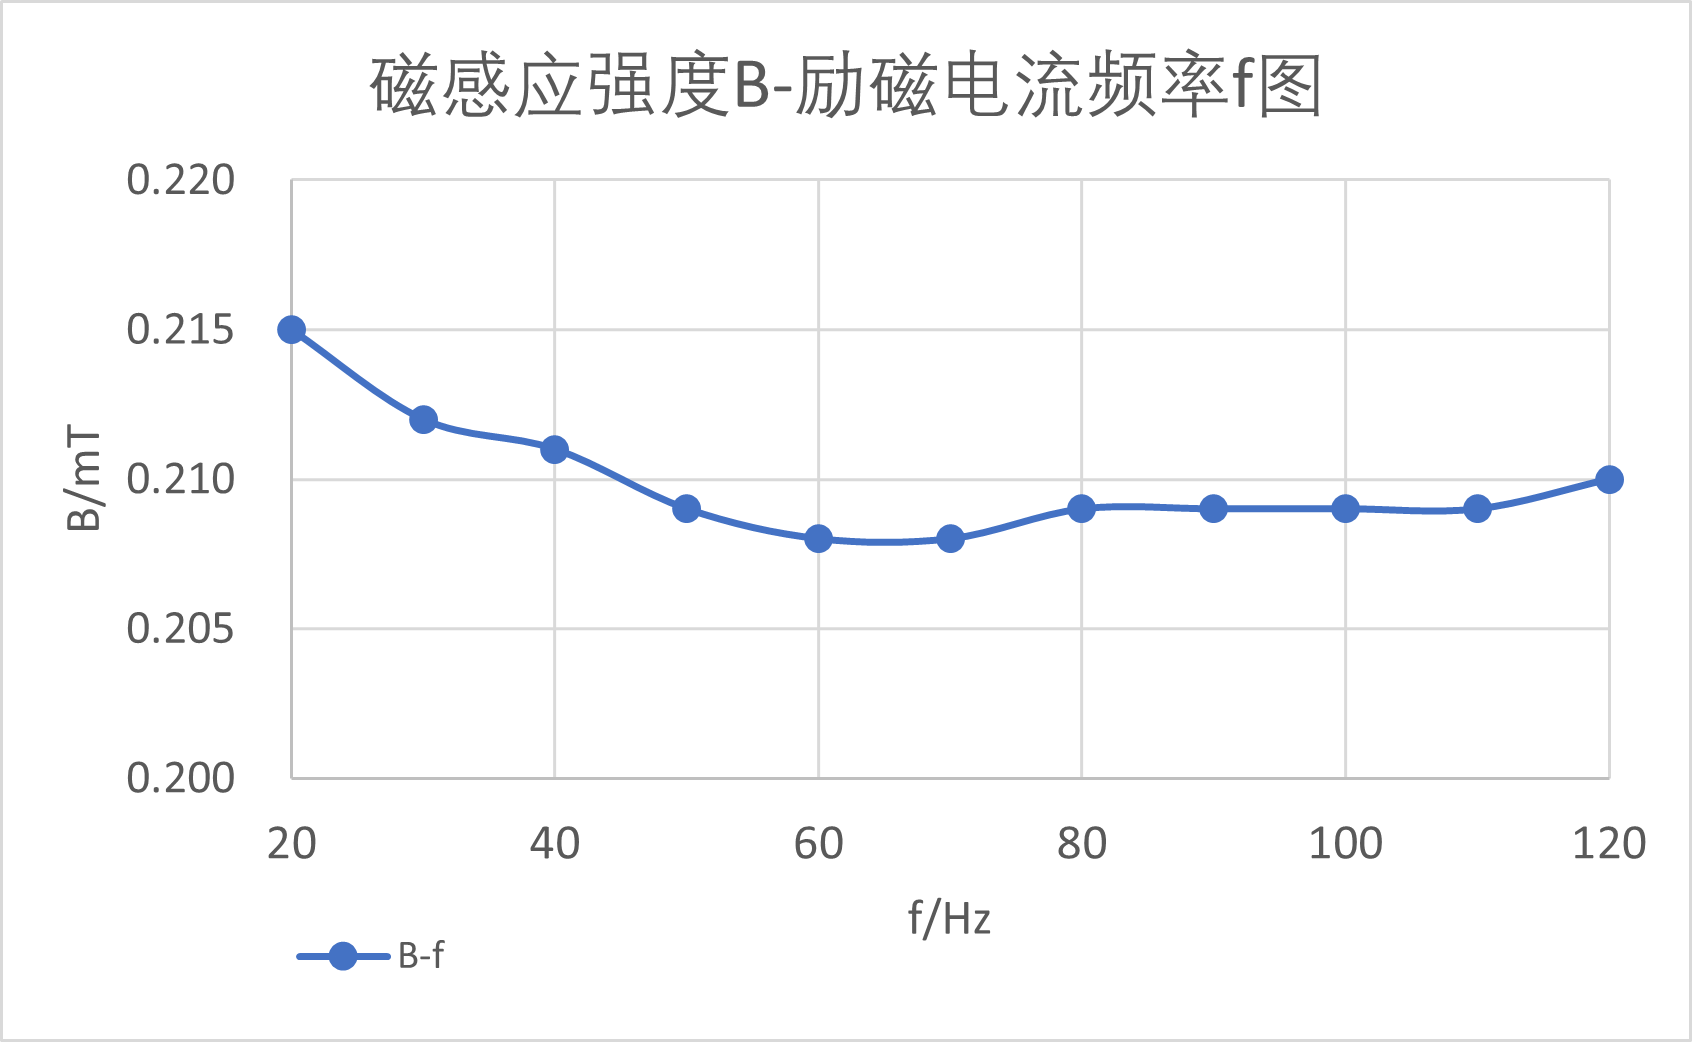
\includegraphics[width=10cm]{Fig/16.png}
    \caption{磁感应强度B-励磁电流频率f图}
    \label{fig:16}
\end{figure}
\par \cref{fig:16}是表\ref{tab:10}数据作图,B基本不随f改变而改变,f增大时B更稳定,测量误差更小。图中的先下降后上升趋势不代表B与f的关系,而为测量误差与计算误差造成的。
\subsection{误差分析}
\begin{enumerate}
    \item \cref{fig:12}中的误差:
    \par \hspace*{2em}在表\ref{tab:9}中,可以看到$0^\circ$和$180^\circ$的读数不一致,也就是探测线圈有测量误差,认为仪器误差为$1-\frac{8.6}{8.7}=1.1\%$以上。实验中,电压读取中有波动,认为波动为$\pm 0.02mV$,产生不确定度$u(U)=\frac{0.02}{6.11}=0.3\%$。移动旋钮时,认为肉眼误差$\pm 0.2mm$,产生测量误差$u(X)=\frac{0.2}{5}=4\%$。
          综合来看,本实验的误差应在5\%以上,实际误差3.3\%,在接受范围内。
    \item \cref{fig:13}和\cref{fig:14}中磁场分布有一到两个点与其他点不同:
    \par \hspace*{2em}本实验中,线圈直径R=105mm=线圈间距a,而实验测量范围为50mm,在测量边缘处理论上不会有磁场的变化。可能的原因是:轴心与刻度0点有区别,中间匀强磁场在边缘会强度降低。
    \item \cref{fig:15}的误差:
    \par \hspace*{2em}实际上本实验误差小,拟合曲线难以看出与原函数$\cos$和$\cos^2$的区别。调整误差为$\pm0.5^\circ$。最大误差$\cos89.5^\circ=0.9\%$。$90^\circ$时磁感应强度不为零,是调整误差和仪器误差共同导致的。外界磁场干扰可忽略。
    \item \cref{fig:16}的误差:
    \par \hspace*{2em}频率较低时,交流对霍尔元件负效应的减弱较小。频率较高时,生成磁场更稳定,测量误差更小。实验中最大误差为$1-\frac{0.208}{0.215}=3.3\%$。
\end{enumerate}
\subsection{思考题}
\begin{enumerate}
    \item 单线圈轴线上磁感应强度的分布规律如何?亥姆霍兹线圈是怎样组成的?其基本条件有哪些?它的磁感应强度分布特点怎样?
    \par \hspace*{2em}实验原理已经叙述。
    \item 探测线圈放入磁感应强度后,不同方向上毫伏表指示值不同,哪个方向最大?如何测准$U_{max}$值?指示值最小表示什么?
    \par \hspace*{2em}理论上$0^\circ$和$180^\circ$同时最大,实际实验数据是$0^\circ$最大。为测准$U_{max}$,在测其之前应该先用实验探究哪个角度探测线圈所得值最大。指示值最小,表示探测线圈方向和磁感应强度方向垂直,磁感应强度在探测线圈法线方向上的分量为最小/0。
    \item 分析圆电流磁感应强度分布的理论值与实验值的误差的产生原因。
    \par \hspace*{2em}误差分析已经叙述。
\end{enumerate}
\begin{center}
    \vspace*{1em}
    \Large \bf 第三部分\qquad 实验反思与实验原始数据
\end{center}
\setcounter{section}{0}
\section{实验反思}
\begin{enumerate}
    \item 本实验操作并不困难。主要操作为旋转旋钮与读数。读数时取最大值会更方便读不稳定的数字。
    \item 实际上,第一部分前期我把电压读数读成了10倍,在计算$K_H$时发现数量级错误才发现,在上面数据表格中进行修正。
    \item 选旋钮慢一点,尊重仪器。
    \item 误差分析与不确定性计算,往往能够解释实验误差的大小之原因。
\end{enumerate}
\section{实验原始数据}
\includepdf[pages={1-3}]{Data/磁场测量实验数据.pdf}
\end{document}